\chapter{Results}
\label{sec:results}

%%%%%%%%%%%%%%%%%%%%% Kurze Einführung %%%%%%%%%%%%%%%%%%%%%

The results of all experimens conducted in this work are described in this chapter.
This chapter's categorization follows the one of the experiments.
First, results of experiments with object detection models are described in \autoref{sec:objectDetectionResults}.
After that results of various cropping mechanisms for inference are depicted in \autoref{sec:autocropResults}.
\autoref{improvedTEPNetResults} gives insights about experiments with different single-frame-based model architectures and \autoref{sec:qualitativeComparison} qualitatively compares the original model of \cite{tepNet2024} with the adapted one.
\autoref{sec:temporalModelsResults} describes results of appraoches that incorporate temporal information to enhance robustness.

%%%%%%%%%%%%%%%%%%%%%%%%%% Object Detection Experiments %%%%%%%%%%%%%%%%%%%%%%%%%%

\section{Object detection Results}
\label{sec:objectDetectionResults}

The first approach is to train object detection models.
For this, the \ac{YOLO}v7 and the \ac{GELAN}-c and \ac{GELAN}-e model versions from \ac{YOLO}v9 are trained.
The best performance scores are obtained from an experiment conducted with the \ac{GELAN}-e model which outperformed the other models in accuracy.
These results are acquired by fine-tuning a model, which is pre-trained on the COCO dataset.
The onlySwitchesLeftRight sub-dataset from RailSem19 is used to train the model (\autoref{sec:usedDatasetsYOLOs}).
\autoref{fig:objectDetectionResultsMetrics} shows performance graphs like the F1 Curve and the Precision-Recall Curve, as well as the confusion matrix with both classes.

\begin{figure}[H]
    \centering
    \begin{subfigure}{0.32\textwidth}
        \centering
        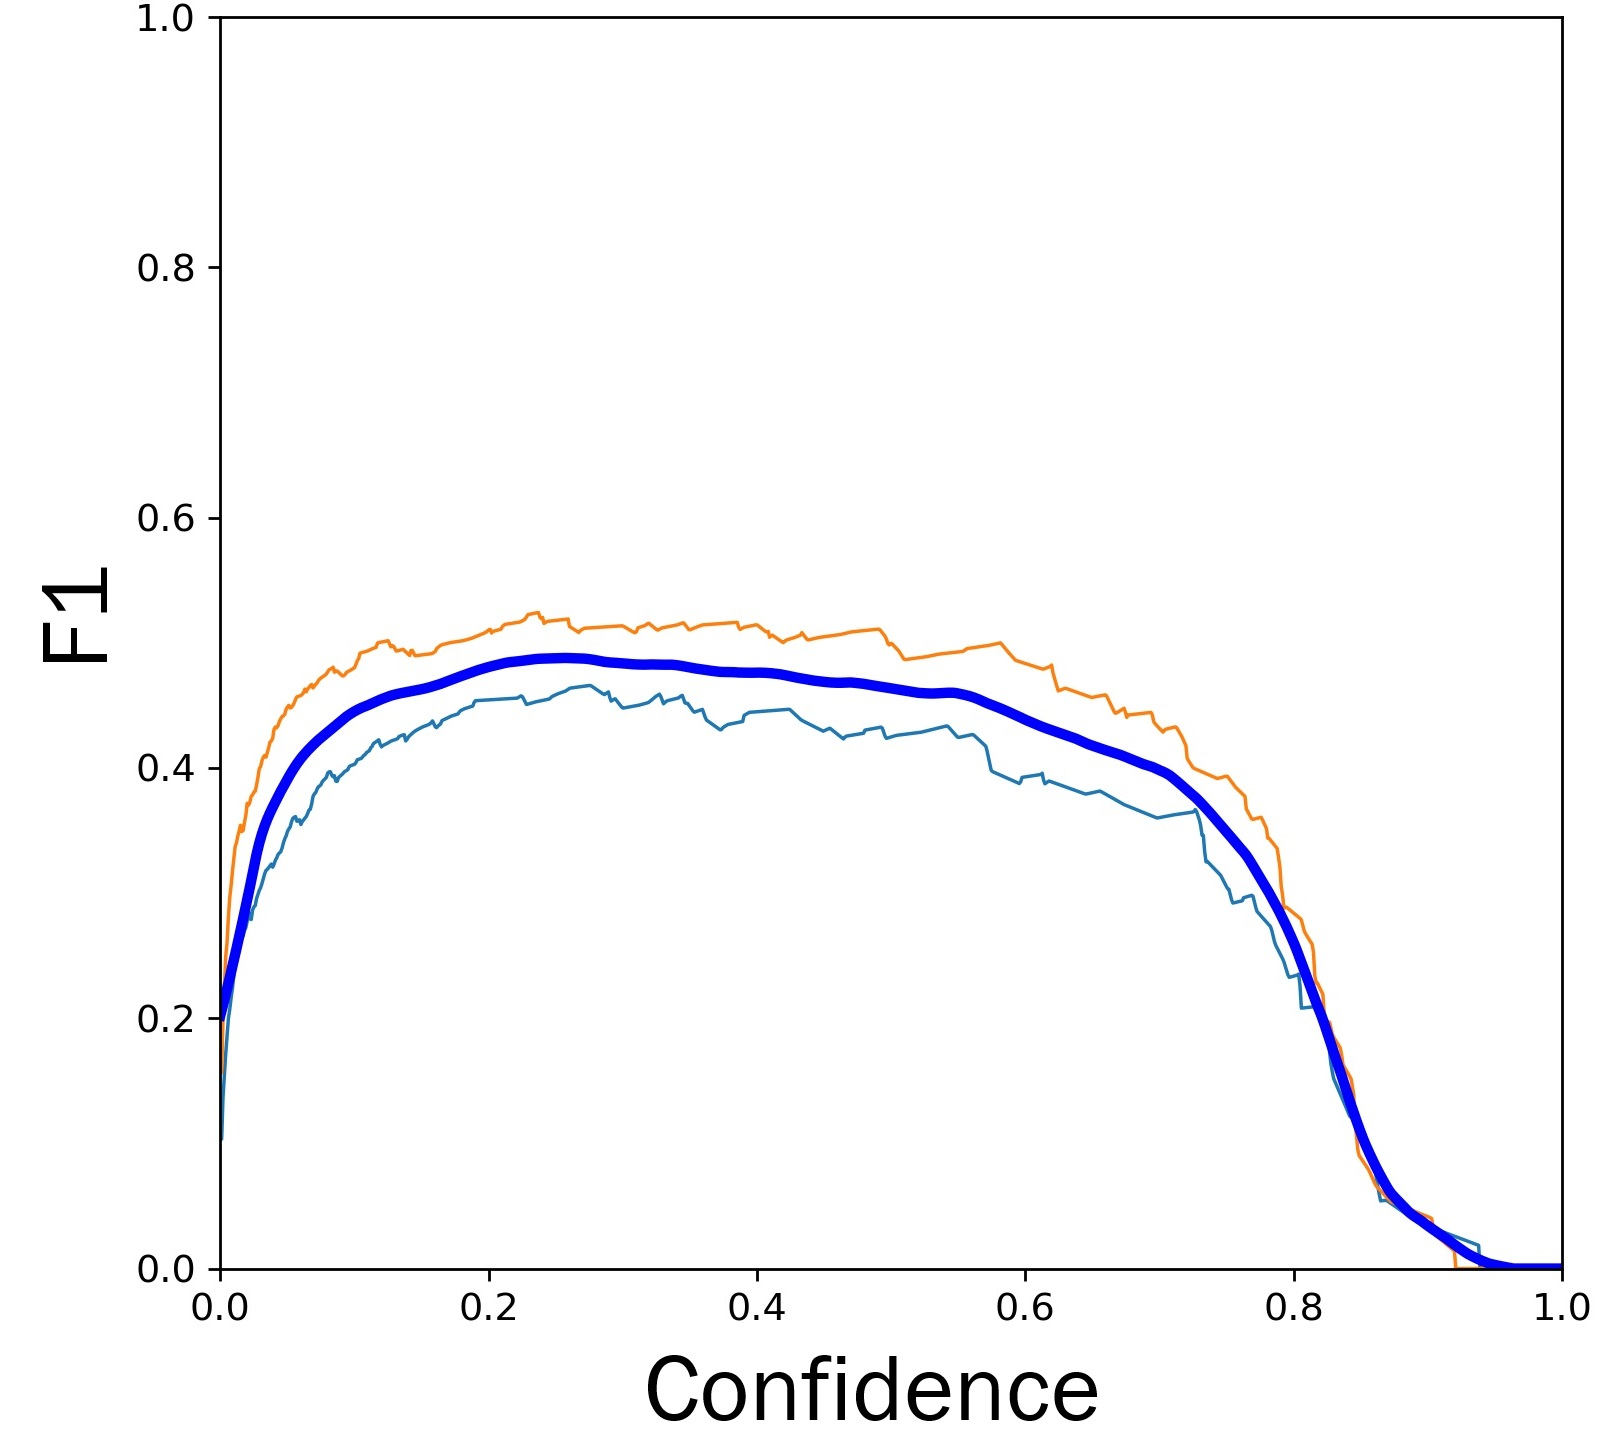
\includegraphics[width=\linewidth,height=4.5cm,keepaspectratio]{PICs/experiments/objectdetectionExperiment/F1_curve_updated.jpg}
        \caption{F1-Confidence Curve}
        \label{fig:objectDetectionResultsMetrics_a}
    \end{subfigure}
    %\hspace*{0.02\textwidth} % Abstand manuell steuern
    \begin{subfigure}{0.32\textwidth}
        \centering
        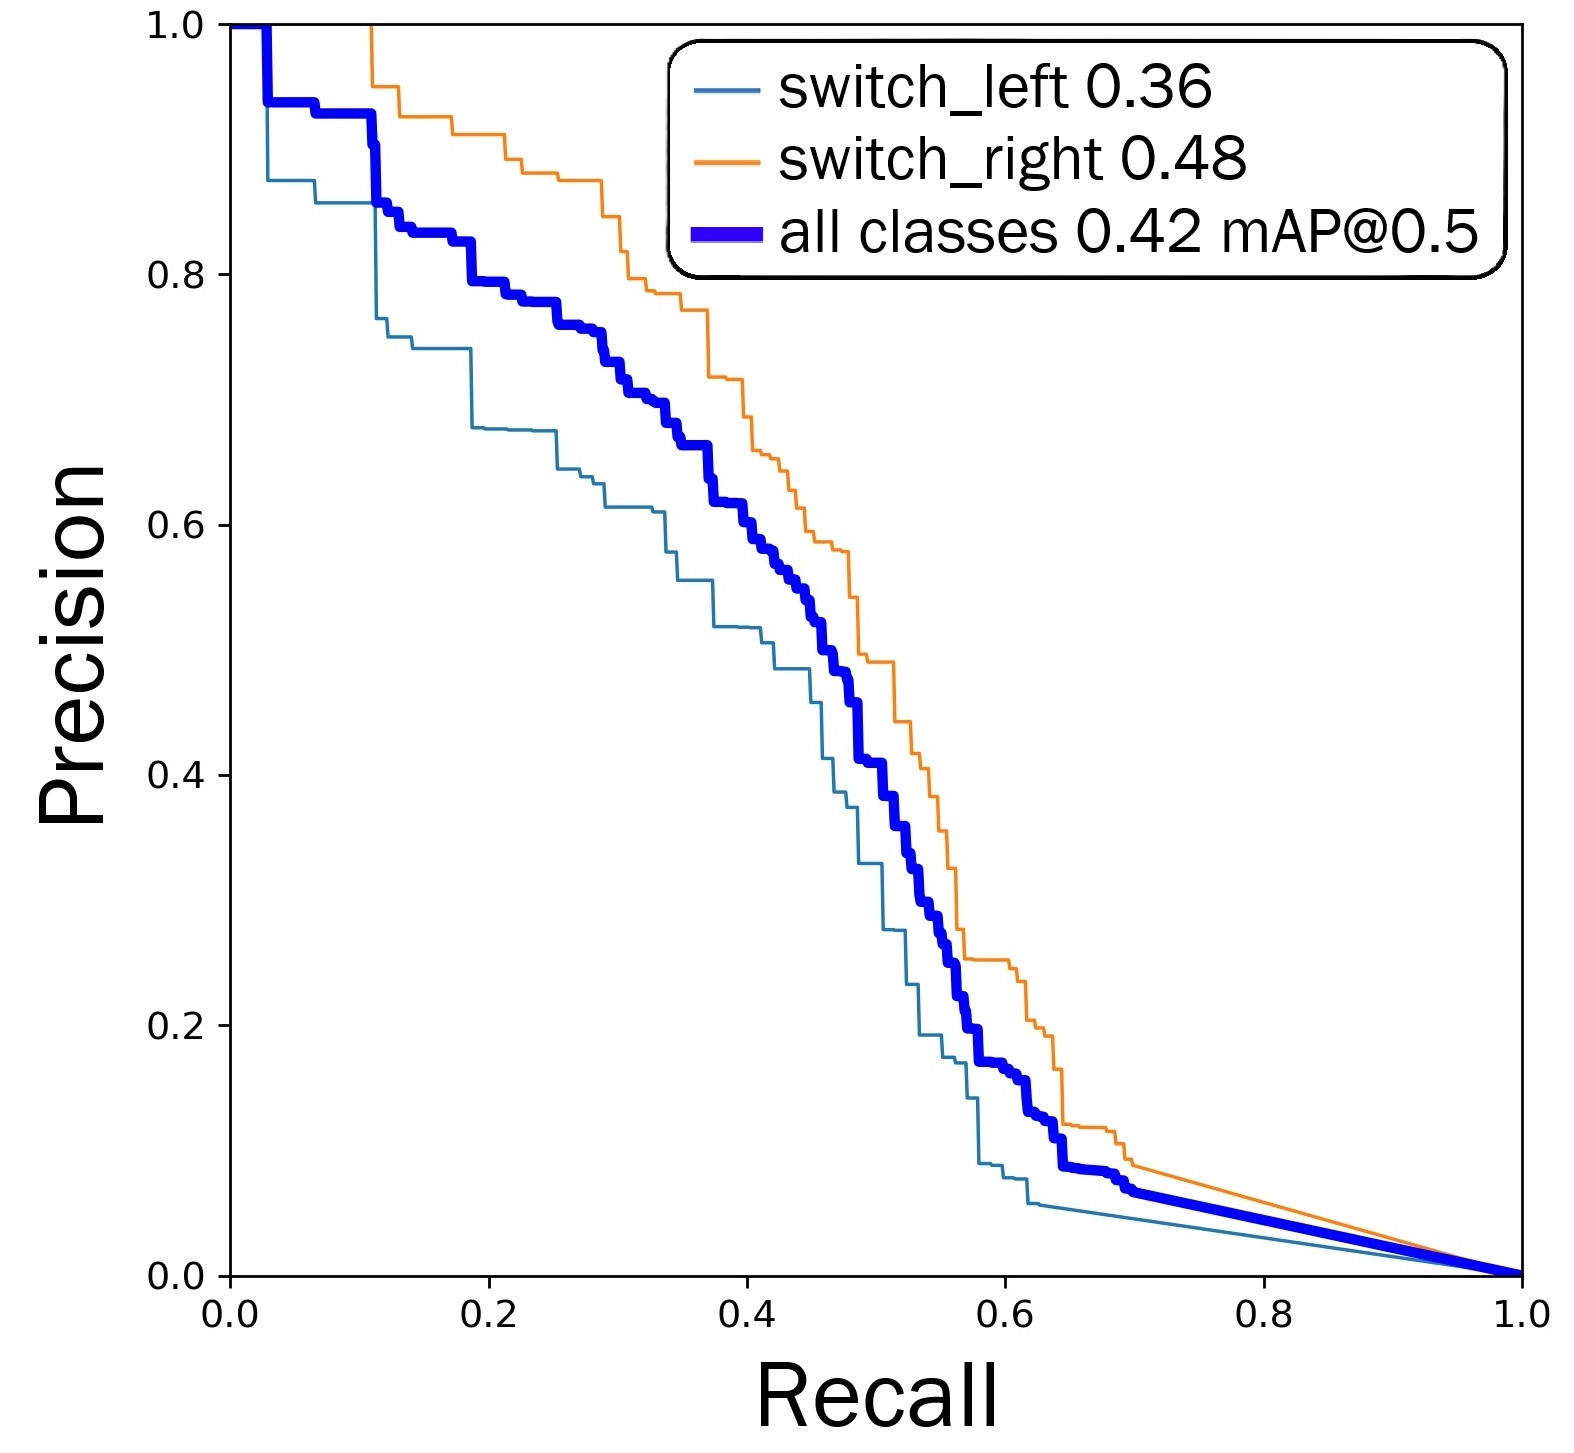
\includegraphics[width=\linewidth,height=4.5cm,keepaspectratio]{PICs/experiments/objectdetectionExperiment/PR_curve_updated.jpg}
        \caption{Precision-Recall Curve}
        \label{fig:objectDetectionResultsMetrics_b}
    \end{subfigure}
    %\hspace*{0.02\textwidth} % Abstand manuell steuern
    \begin{subfigure}{0.32\textwidth}
        \centering
        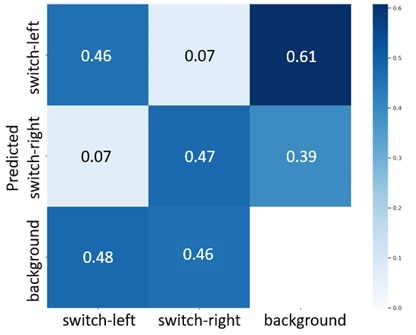
\includegraphics[width=\linewidth,height=4.5cm,keepaspectratio]{PICs/experiments/objectdetectionExperiment/confusion_matrix_updated.jpg}
        \caption{Confusion Matrix}
        \label{fig:objectDetectionResultsMetrics_c}
    \end{subfigure}
    \caption{Results of best-performing object detection model experiment: \ac{GELAN}-e fine-tuned on onlySwitchesLeftRight and pre-trained on COCO.
    Thin Orange lines are $switch\_right$ labels, thin blue lines are $switch\_left$ labels and thick blue lines are all classes}
    \label{fig:objectDetectionResultsMetrics}
\end{figure}

However, as visualized in \autoref{fig:objectDetectionResultsMetrics} the Precision-Recall Curve and the F1 Curve show unsatisfying results.
The confusion matrix also indicates that the model's prediction performances are below 50\% for both classes.
The reason for that presumably lies in the complexity of the task.
Switches look similar to rails and predicting switch states further increases the difficulty, because the only difference is the start of the switch.
Additionally, the \ac{GT} bounding boxes of most switch labels are very small.
As shown in \autoref{fig:annotationAnalysis} most crops have widths of about 0.02 and heights of about 0.015 relative to the dataset images.
Converted into pixels with the image resolution of $1920 \times 1080$, this results into crops with heights around 22 pixels and widths around 29 pixels.
RailSem19 \cite{railsem19dataset} also states that this task is difficult.
In one of their experiments, they only considered the crops of $switch\_left$ and $switch\_right$ labels and turned it into a classification task.
Even after they expanded the crops vertically by 125\% and horizontally by 30\% to increase the context, they had many images with dimensions below 28 pixels.
After dropping those and training a denseNet161, the accuracy only achieved 67\%.

\begin{figure}[H]
    \centering
    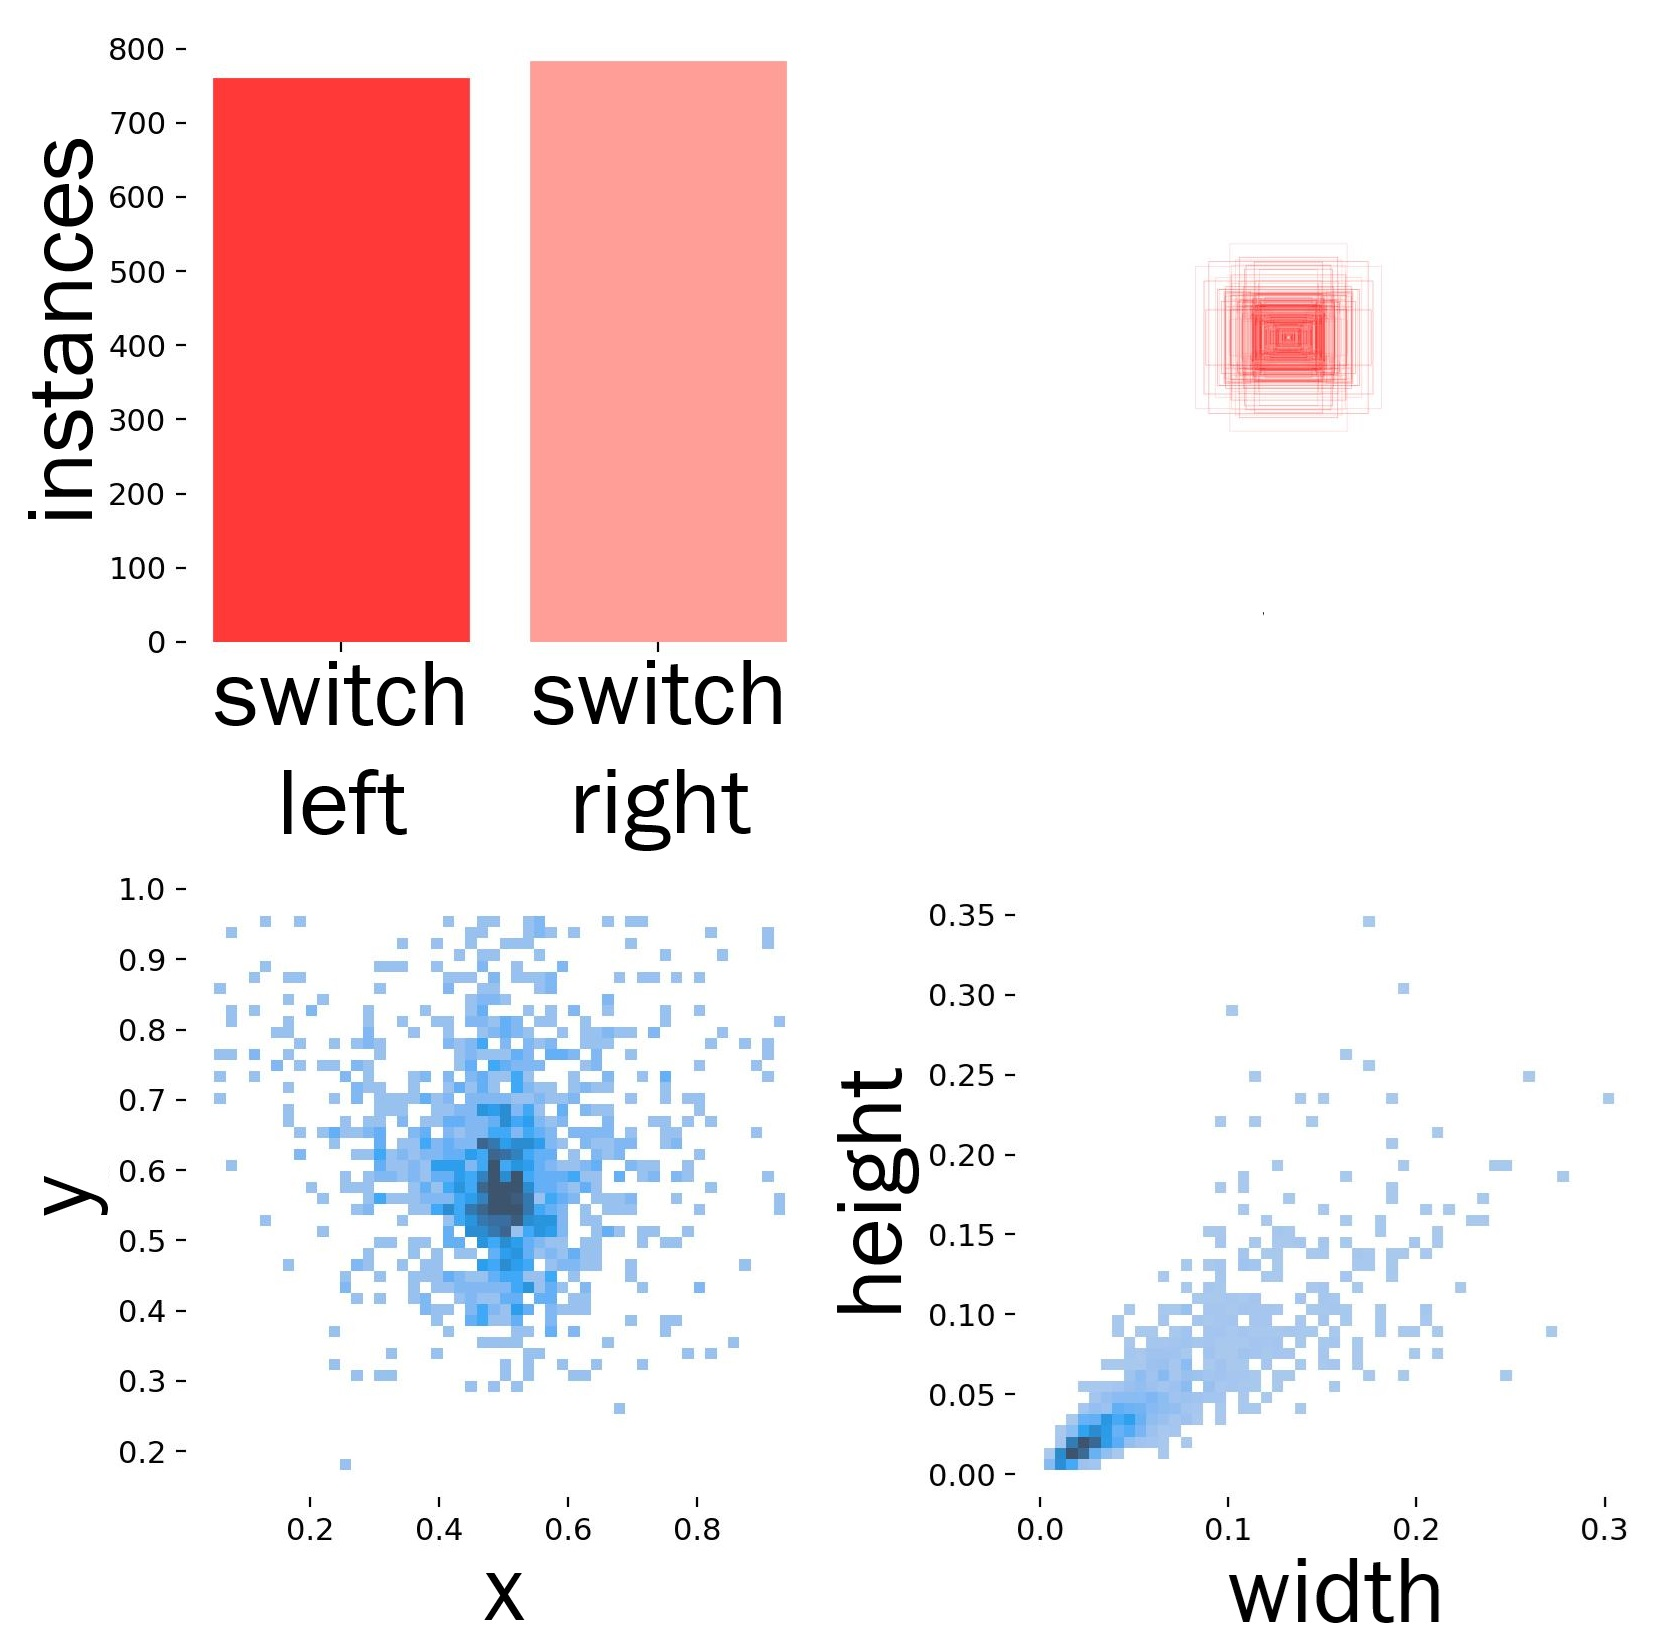
\includegraphics[width=0.6\linewidth]{PICs/experiments/objectdetectionExperiment/labels_updated.jpg}
    \caption{Annotation analyses of \ac{YOLO}v9 \cite{YOLOv9GitHub}. In the lower two graphs the axis are relativ to the image dimensions.}
    \label{fig:annotationAnalysis}
\end{figure}

Because of the complexity of this task and the unsatisfactory results it cannot be assumed switch states are correctly predicted.
Therefore the approach of predicting the direction of the train with an object detection model is discarded.
A fundamentally different approach must be found, making further experiments with semantic segmentation models unnecessary.

%%%%%%%%%%%%%%%%%%%%%%%%%% Improved Autocropper %%%%%%%%%%%%%%%%%%%%%%%%%%

\section{Autocrop Results}
\label{sec:autocropResults}

For the improved auto cropping mechanism there are many different versions implemented in this work.
All of them have been evaluated on the Switch evaluation dataset.
Even though the cropping mechanism is primarily designed for the inference of videos, performance differences can be recorded in this dataset.
The track of each image is predicted 50 times and the crop coordinates are adjusted iteratively.
The results of autocrop versions are shown in \autoref{tab:autocropResults}.

\begin{table}[H]
    \centering
    \begin{tabular}{|l|c|c|c|c|c|}
    %\begin{tabular}{| p{0.3\linewidth} | p{0.6\linewidth} |}
        \hline
        \textbf{used Methods} & \textbf{original \cite{tepNet2024}} & \textbf{Version 2} & \textbf{Version 3} & \textbf{Version 4} & \textbf{Version 5}\\
        \hline
        RA                                 & \checkmark &            &            &            &            \\
        \hline
        EMA                                &            & \checkmark & \checkmark & \checkmark & \checkmark \\
        \hline
        reset rule [40\%] $(\frac{1}{3}, \frac{1}{2}, \frac{2}{3})$  &            & \checkmark & \checkmark & \checkmark & \checkmark \\
        \hline
        aspect ratio (16:9)   	           &            &            & \checkmark &            &            \\
        \hline
        aspect ratio (1:1)                 &            &            &            & \checkmark &            \\
        \hline
        10\% at the start                  &            &            &            &            & \checkmark \\
        \hline
        Switch evaluation dataset          & 88.97\%    & \textbf{91.18\%} & 86.76\% & 91.18\% & 90.44\%    \\
        \hline
    \end{tabular}
    \caption{Various versions of autocrops evaluated on the Switch evaluation dataset.
    Models predict each image 50 times and adjust the autocrop iteratively.
    Version 2 includes multiple experiments with different parameters for the reset rule.
    Since the evaluation dataset consists of images and the reset rule is applied in video sequences, only the best-performing parameters are included in this table.}
    \label{tab:autocropResults}
\end{table}

\noindent An improvement in accuracy can be observed in all versions but version 3.
In Version 3, the crop is forced to be in a 16:9 aspect ratio.
It is assumed that this ratio presents a disadvantage since the crop is resized in a quadratic 512 $\times$ 512 image afterward.
This assumption is supported by Version 4 also achieving the highest score.
This version has a fixed quadratic aspect ratio.
Version 5 is very similar to Version 2 but instead of starting with the whole image, its initial crop coordinates are set to $(0, 0.1 \times image\_height, 1)$.
The whole image width but only the lowest 10\% of the image are considered.
This proves to be effective in some cases, resulting in a much quicker convergence to a desired crop.
However, it also shows that it is highly situational dependent.
Version 5 works better than starting with the whole image only when a single track is visible in the beginning.
In starting scenarios with at least two tracks the model struggles to find the right one. Therefore the use of Version 5 is not recommended.
Version 2 and 4 are the highest-performing methods.
However, for this work Version 2 is used for further experiments because it does not introduce additional heuristics like Version 4.
Therefore, it is more independent of scene situations.

The parameters of the reset rule, such as the allowed percentage by which the prediction can descend and the crop coordinates to which the crop is reset, are determined based on the observed behavior of the models in various scenarios.
These parameters are described in \autoref{sec:autocropExperiments} in more detail.
In uncertainty, all Models have receding horizon lines, even though different backbones are used.
Therefore the crop is reset when the prediction is below 40\% of the crop height.
Thresholds of 30\% 40\%, 50\%, and 60\% are tested.
With 50\% and 60\%, the crop is sometimes reset even though the prediction is correct, and with 30\% the convergence takes too much time.
Therefore 40\% is chosen to be the threshold.
The crop is reset to $(\frac{1}{3}, \frac{1}{2}, \frac{2}{3})$.
These parameters are near the optimal crop coordinates for all test scenarios without narrowing the crop too much, which would lead to a possible collapse.

\vspace{0.5cm}

\noindent To qualitatively show the difference between the original auto crop from \cite{tepNet2024} and the proposed one for this work, both are tested on a difficult scenario.
A video from a train driving through a railroad station with many rails, switches, and crossings is chosen to evaluate the different auto-crop mechanisms to their cores.
Additionally, the ResNet18 backbone is used because it is the worst-performing one in terms of accuracy and differences can be observed more easily.


\begin{figure}[H]
    \centering

    % Unteres Grid mit kleineren Bildern
    \begin{minipage}{0.195\textwidth}
        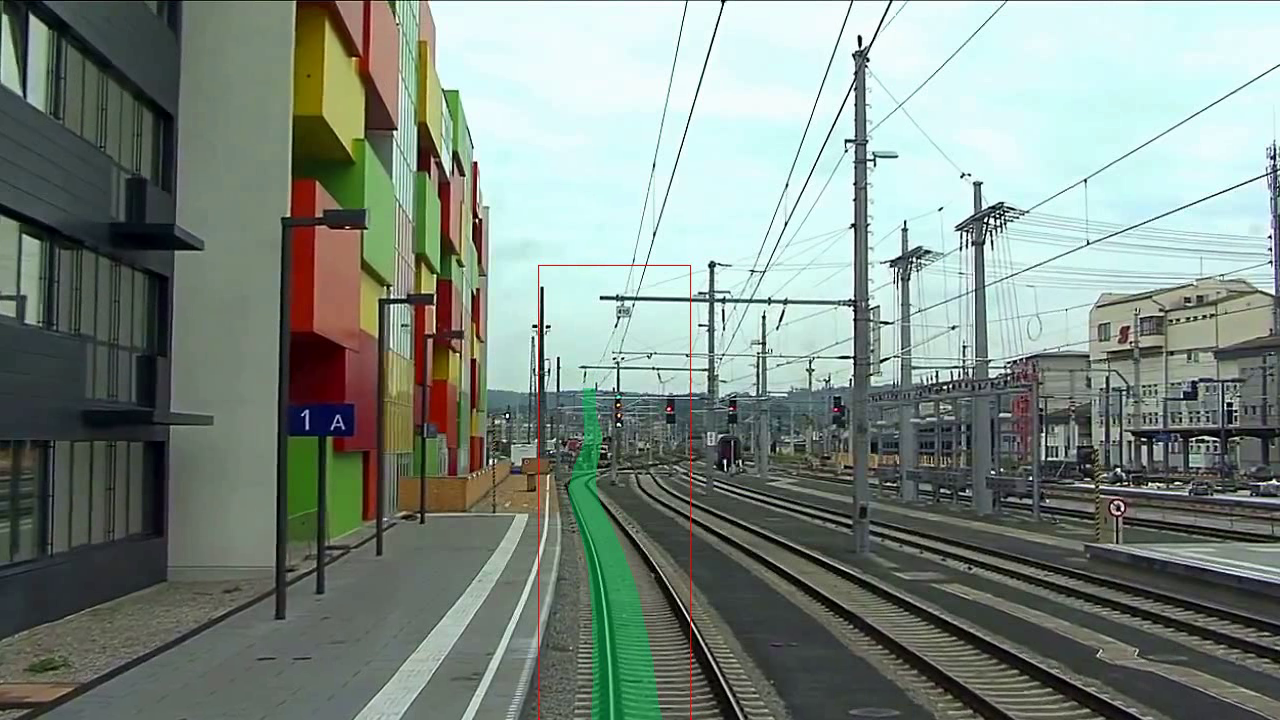
\includegraphics[width=\textwidth]{PICs/experiments/autocropExperiments/output_frames/frame_100.png}
    \end{minipage}
    \hfill
    \begin{minipage}{0.195\textwidth}
        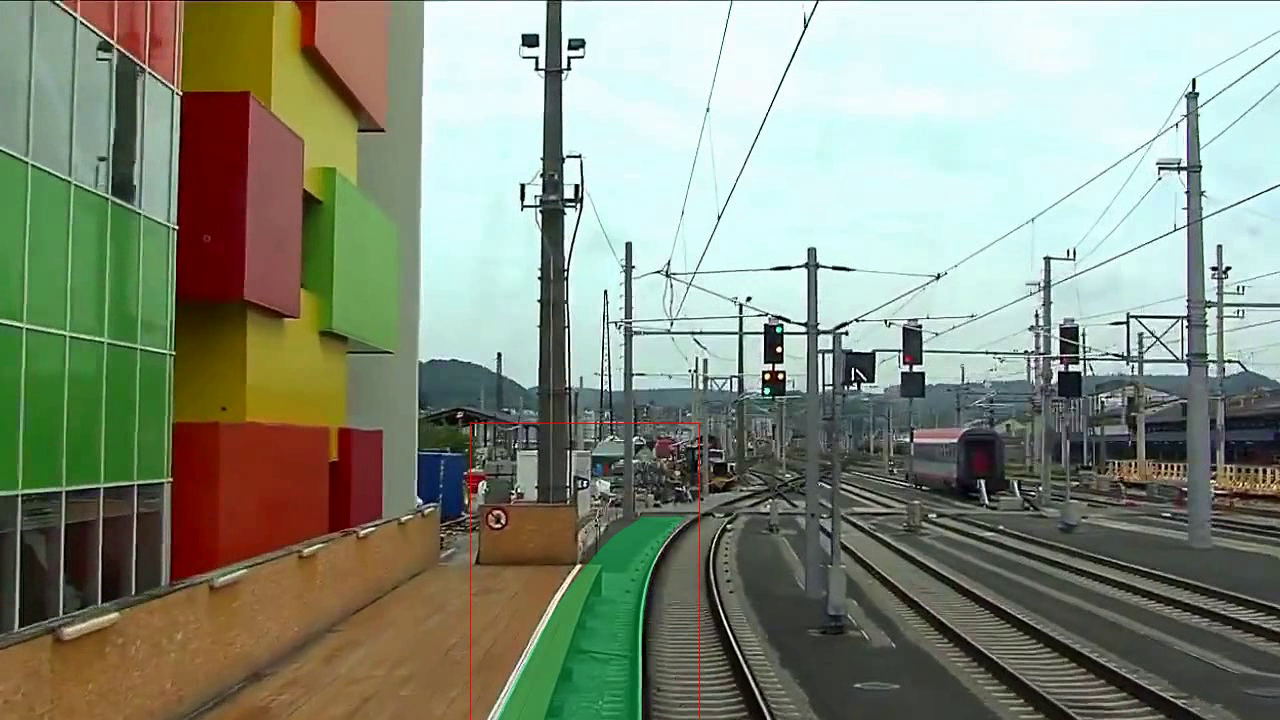
\includegraphics[width=\textwidth]{PICs/experiments/autocropExperiments/output_frames/frame_700.png}
    \end{minipage}
    \hfill
    \begin{minipage}{0.195\textwidth}
        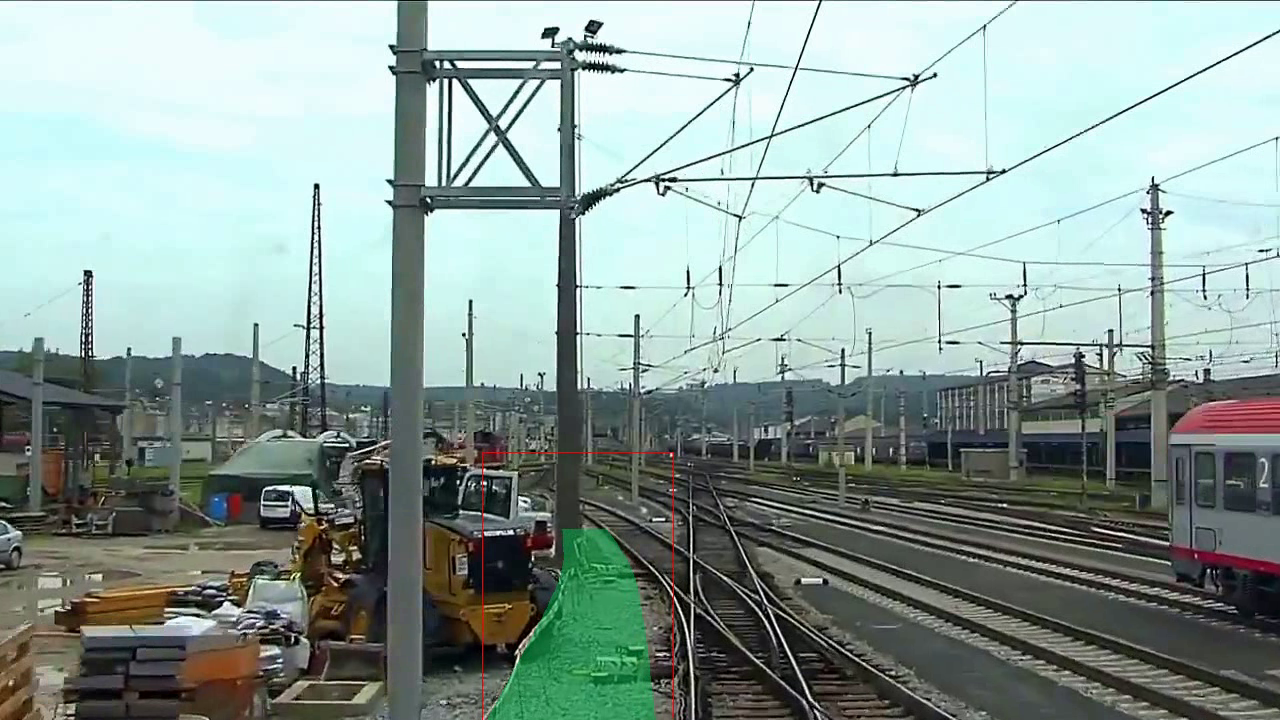
\includegraphics[width=\textwidth]{PICs/experiments/autocropExperiments/output_frames/frame_1000.png}
    \end{minipage}
    \hfill
    \begin{minipage}{0.195\textwidth}
        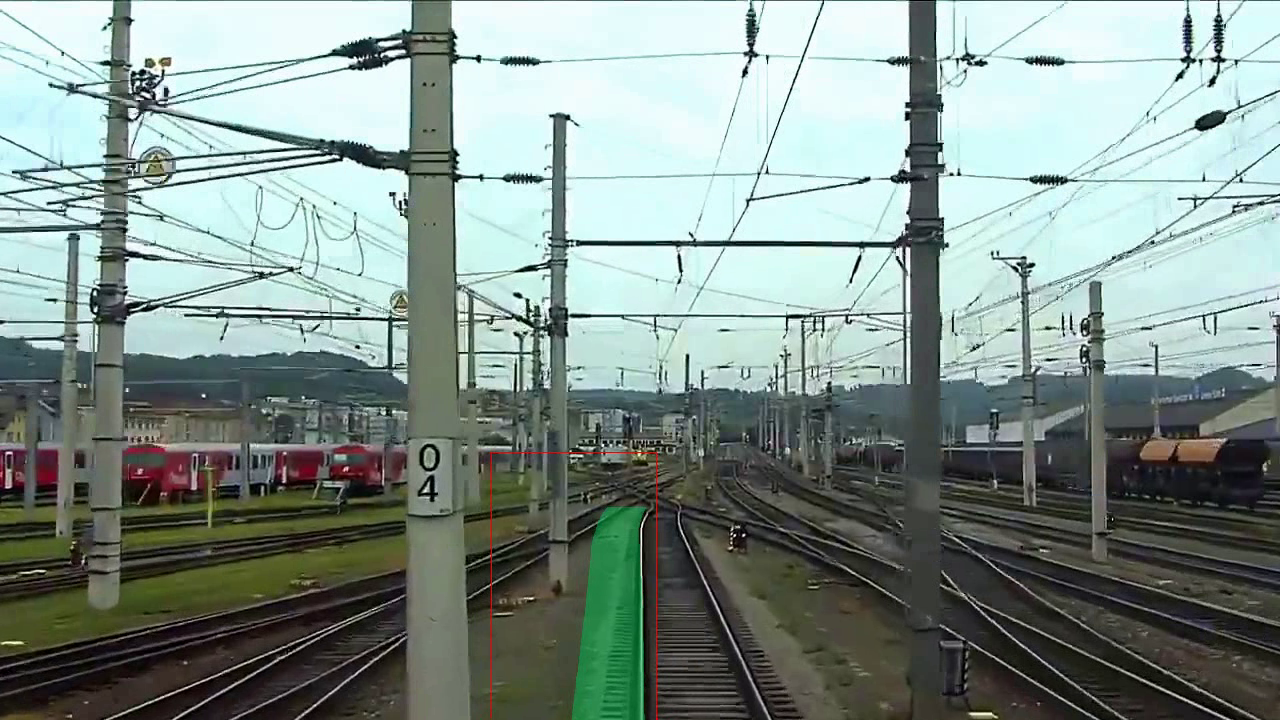
\includegraphics[width=\textwidth]{PICs/experiments/autocropExperiments/output_frames/frame_1600.png}
    \end{minipage}
    \hfill
    \begin{minipage}{0.195\textwidth}
        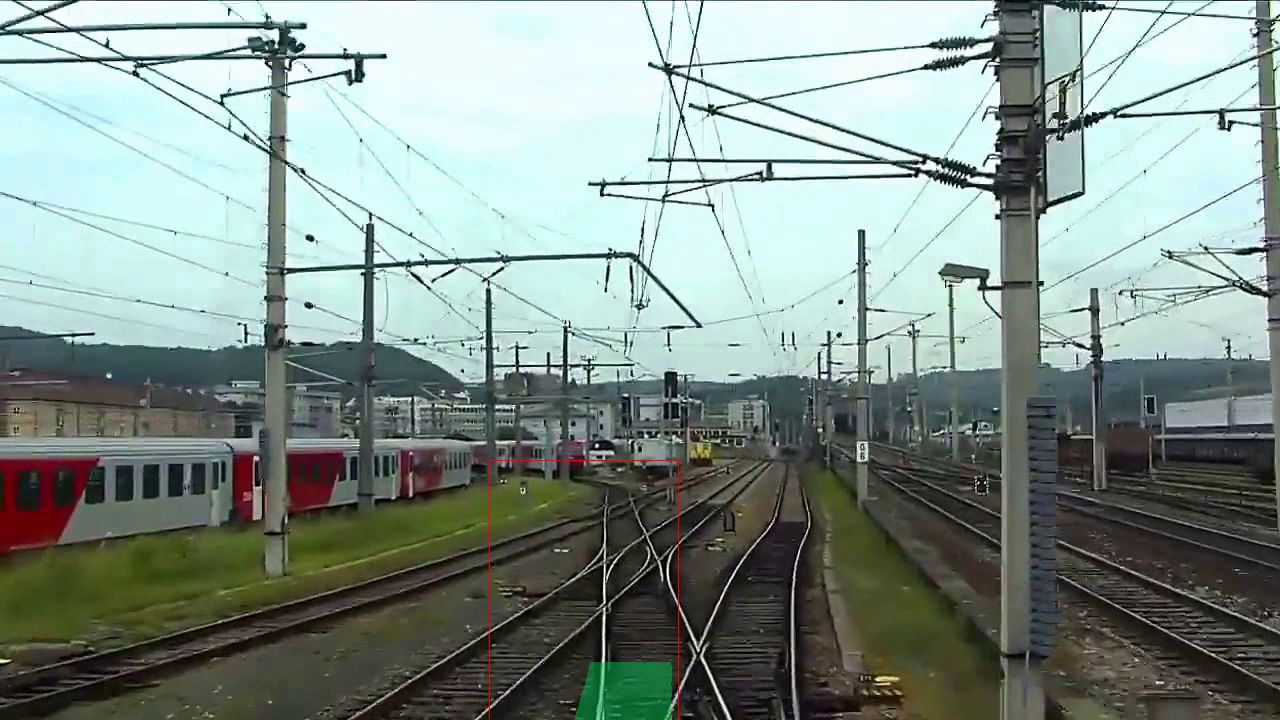
\includegraphics[width=\textwidth]{PICs/experiments/autocropExperiments/output_frames/frame_1900.png}
    \end{minipage}

    % Unteres Grid mit kleineren Bildern
    \begin{minipage}{0.195\textwidth}
        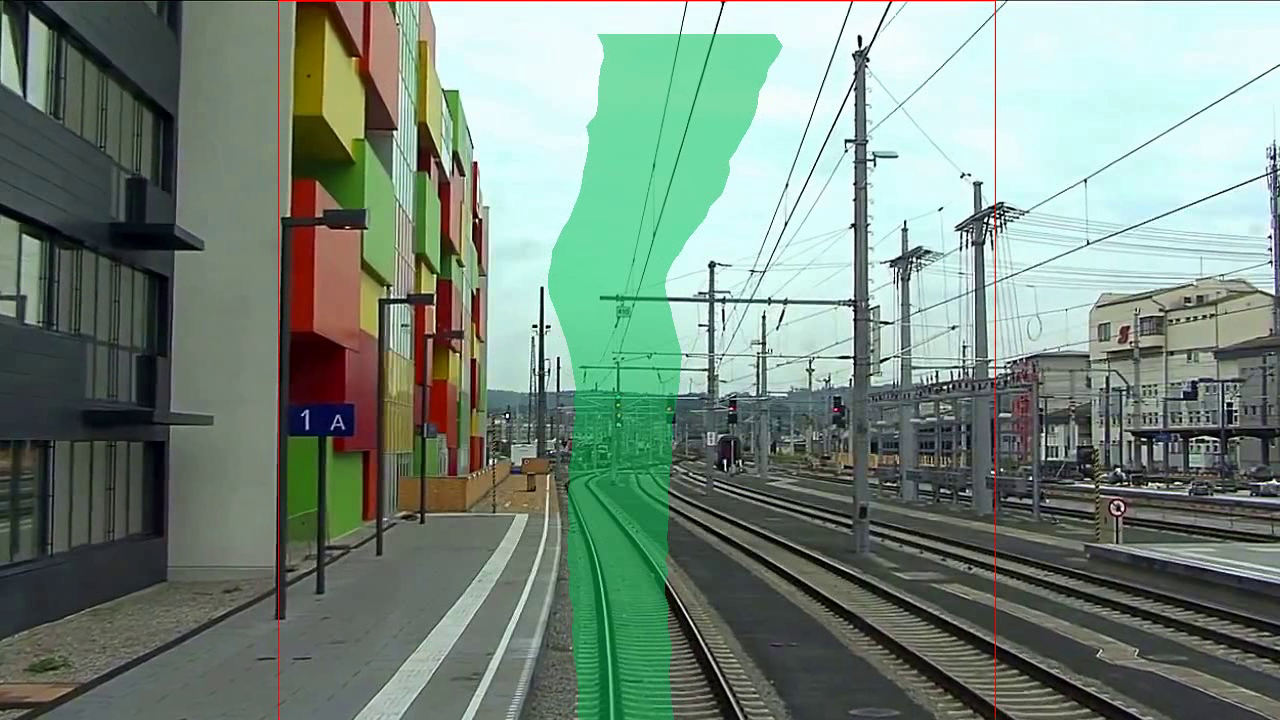
\includegraphics[width=\textwidth]{PICs/experiments/autocropExperiments/output_frames_improved/frame_100.png}
    \end{minipage}
    \hfill
    \begin{minipage}{0.195\textwidth}
        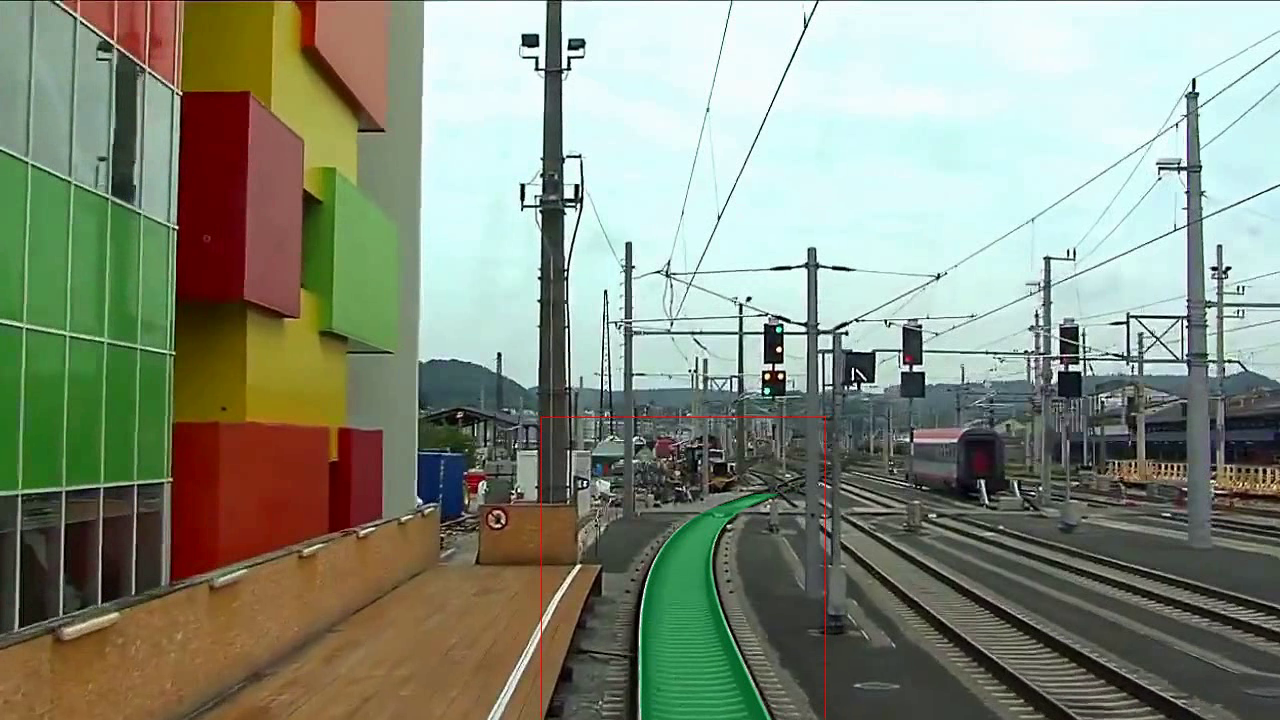
\includegraphics[width=\textwidth]{PICs/experiments/autocropExperiments/output_frames_improved/frame_700.png}
    \end{minipage}
    \hfill
    \begin{minipage}{0.195\textwidth}
        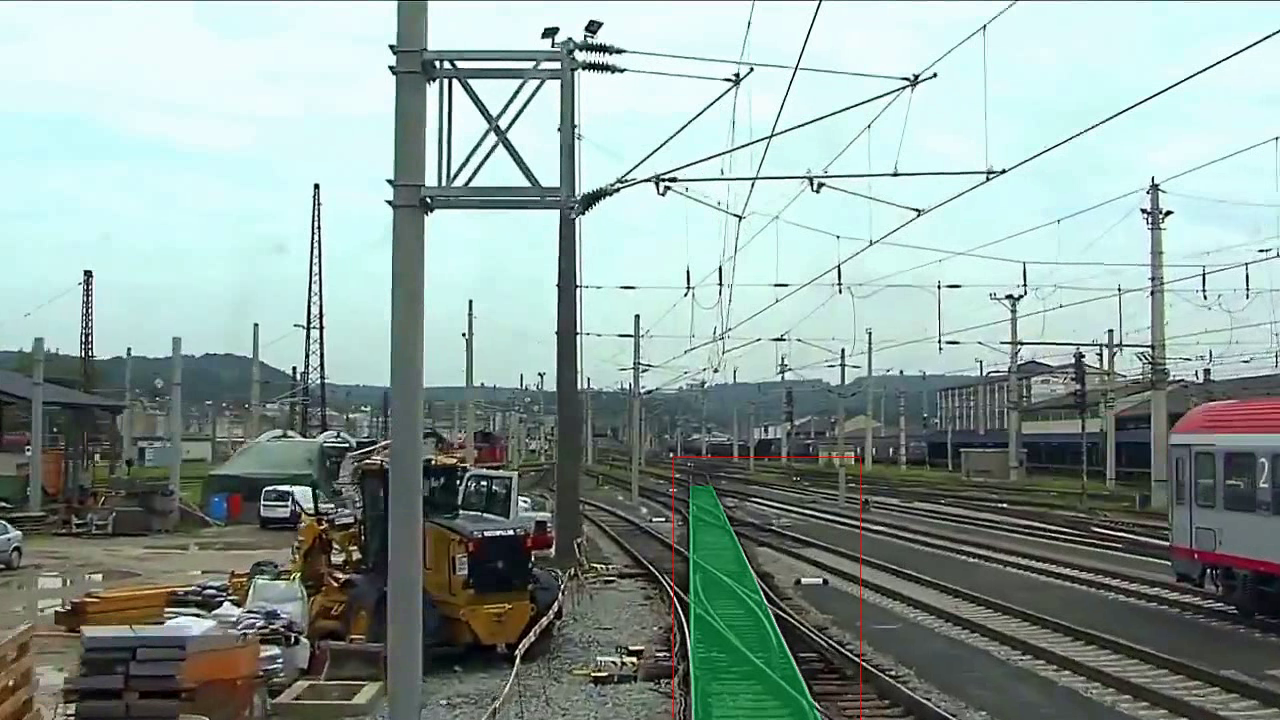
\includegraphics[width=\textwidth]{PICs/experiments/autocropExperiments/output_frames_improved/frame_1000.png}
    \end{minipage}
    \hfill
    \begin{minipage}{0.195\textwidth}
        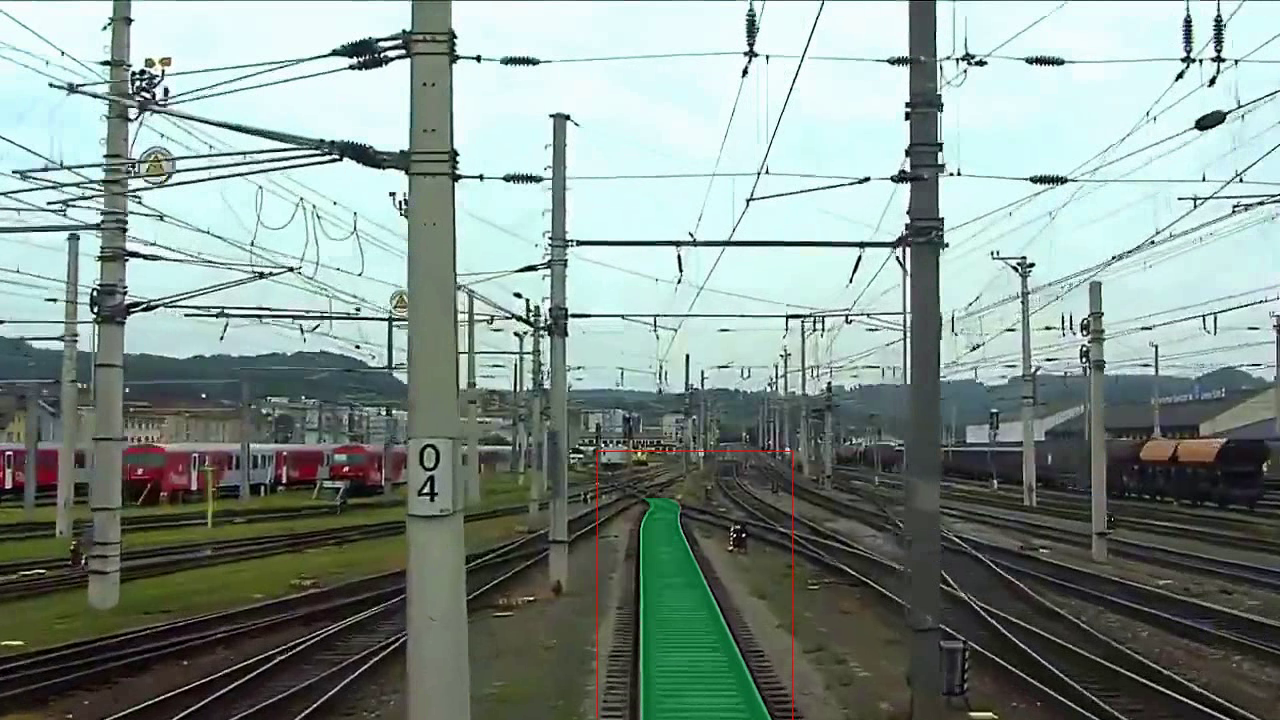
\includegraphics[width=\textwidth]{PICs/experiments/autocropExperiments/output_frames_improved/frame_1600.png}
    \end{minipage}
    \hfill
    \begin{minipage}{0.195\textwidth}
        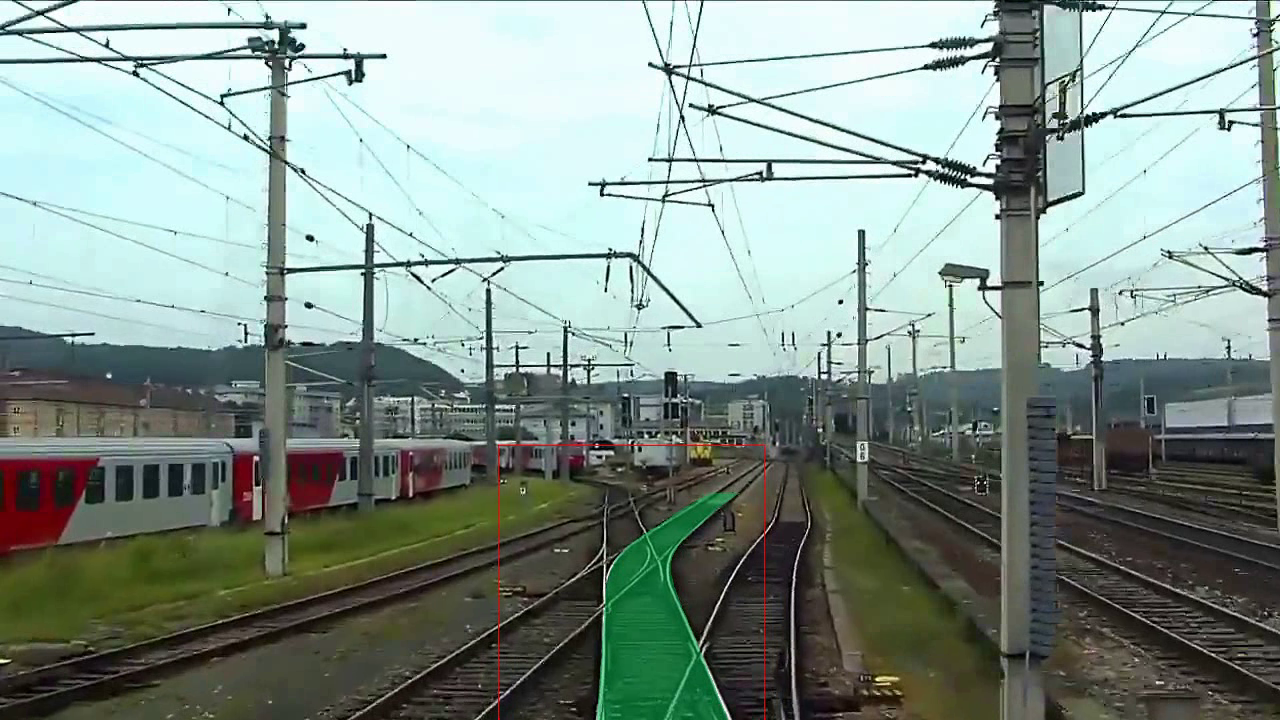
\includegraphics[width=\textwidth]{PICs/experiments/autocropExperiments/output_frames_improved/frame_1900.png}
    \end{minipage}

    % Vierte Reihe für die Zeitachse
    \begin{minipage}{1.0\textwidth}
        \centering
        \begin{tikzpicture}
            % Zeit "Time" über dem Pfeil links positionieren
            \node at (-7.5, 0.3) {time}; % Text "Time"
            \draw[-Stealth, thick] (-8, 0) -- (8, 0); % Pfeil von ganz links nach ganz rechts
        \end{tikzpicture}
    \end{minipage}

    % Beschriftung unter dem Grid
    \vspace{0.5cm}
    \caption{Comparison between the original and the adapted auto-crop including frames 100, 700, 1000, 1600, and 1900 of the evaluation video \cite{temporalDataset_youtube_video}.
    The first row is the original auto-crop from \cite{tepNet2024} and the second row is the proposed one.}
    \label{fig:autocropVideoComparison}
\end{figure}

\begin{figure}[H]
    \centering
    \begin{subfigure}{\textwidth}
        \centering
        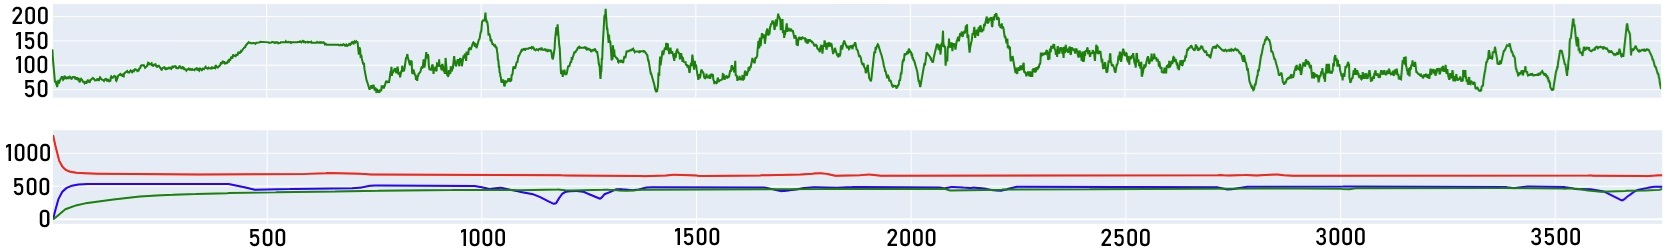
\includegraphics[width=\textwidth]{PICs/experiments/autocropExperiments/original_updated.jpg} % erstes Bild
        \caption{Original auto-crop mechanism}
        \label{fig:autocropResultsTrends_a}
    \end{subfigure}
    %\hspace*{0.02\textwidth} % Abstand manuell steuern
    \begin{subfigure}{\textwidth}
        \centering
        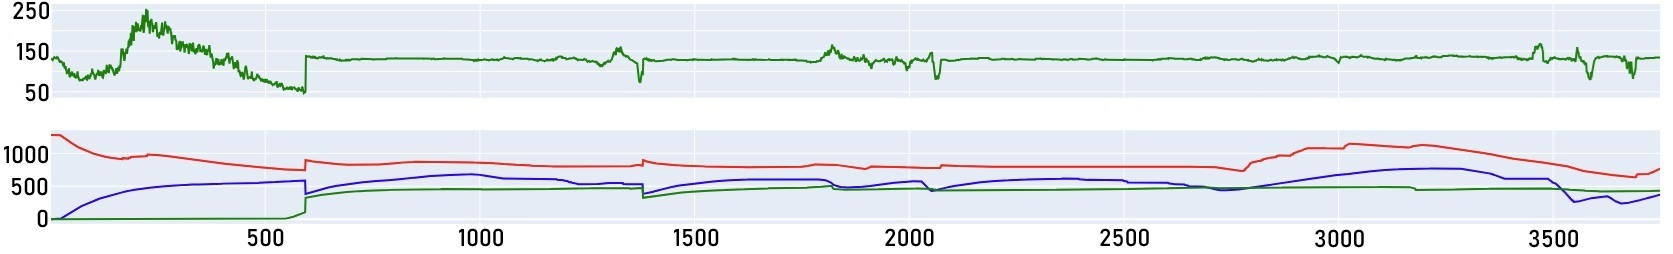
\includegraphics[width=\textwidth]{PICs/experiments/autocropExperiments/improved_updated.jpg} % zweites Bild
        \caption{Adapted auto-crop mechanism (Version 2)}
        \label{fig:autocropResultsTrends_b}
    \end{subfigure}
    \caption{Trend of the evaluation video \cite{temporalDataset_youtube_video} shown in \autoref{fig:autocropVideoComparison}.
    The first and third graphs with a single green line show the rail width at the first anchor line.
    The second and fourth graphs show crop coordinates (blue=left, red=right, green=top).
    Jumps in graphs from the adapted mechanism indicate resets, like the one at around frame 600.
    It also shows that with the original technique, cropcoords are stable and the prediction is not and the improved auto-crop reverses this relationship.}
    \label{fig:autocropResultsTrends}
\end{figure}


\noindent Models with a ResNet18 backbone show an additional behavior when uncertain.
The width of the predicted track becomes unstable, especially at the first few anchors.
This is because the camera is in a fixed position in this video \cite{temporalDataset_youtube_video}, and when correctly predicting the track, the width does not change at the bottom of the image.
Therefore, the track width at the first anchor line is a good indicator of uncertainty.
\autoref{fig:autocropVideoComparison} and \autoref{fig:autocropResultsTrends} show the evaluation of a model with the ResNet18 backbone on the evaluation video \cite{temporalDataset_youtube_video}.
\autoref{fig:autocropVideoComparison} shows the frames 100, 700, 1000, 1600, and 1900.
\autoref{fig:autocropResultsTrends} visualizes the trend of track width and crop coordinates.

As shown in frame 100, both models need time to find the right track.
The unstable rail width of both models also indicates this.
\autoref{fig:autocropResultsTrends_b} displays a jump of cropcoords and rail width at around frame 600, indicating a reset.
After that, the adapted auto-crop mechanism proves to be correct and stable.
However, in the video with the original cropping mechanism, the crop converges to an area that does not include the rail.
Since the system does not include a reset rule, it cannot recover from the mistake at the start.
When comparing both techniques in a broader scope, the original cropping mechanism shows stable crop coordinates, but the prediction is often incorrect.
On the other hand, the adapted technique moves more freely and quickly adapts to challenging scenarios.
Consequently, the prediction becomes more stable, which is the desired output.

%%%%%%%%%%%%%%%%%%%%%%%%%% Improved TEP-Net %%%%%%%%%%%%%%%%%%%%%%%%%%

\section{Improved TEP-Net}
\label{improvedTEPNetResults}

This chapter describes the results of all experiments aiming to improve the single-frame-based model of \cite{tepNet2024}.
First, the results of using various backbones are described.
The following subchapter depicts how true pooling layers affect performance.
After that, the results of experiments with different prediction heads are described.
Each subchapter builds on the previous one, resulting in a final improved single-frame-based model.

\subsection{Backbones}

\begin{table}[H]
    \centering
    \resizebox{\textwidth}{!}{
        \begin{tabular}{lcccccc}
            \hline
            \rowcolor{white} \textbf{Model} & \textbf{Parameters} & \textbf{Flops} & \textbf{MACs} & \textbf{Latency TRT FP32 / FP16} & \textbf{IoU} & \textbf{Switch Eval} \\
            \hline
            \rowcolor[gray]{0.9} ENB3 \cite{tepNet2024} & 14.57M & 9.74B          & 5.16G          & 24.89 / 15.26 ms        & \textbf{97.53 \%} & 91.18 \% \\ 
            \rowcolor{white}     RN18 \cite{tepNet2024} & 15.64M & 18.98B         & 9.53G          & 9.48 / 3.25 ms          & 96.95 \%          & 80.15 \% \\ 
            \hline
            \rowcolor[gray]{0.9} MNV3-Small & \textbf{5.33M}     & \textbf{0.55B} & \textbf{0.30G} & \textbf{3.13 / 2.05 ms} & 96.19 \%          & 73.53 \% \\ 
            \rowcolor{white}     MNV3-Large & 7.27M              & 2.15B          & 1.17G          & 6.41 / 3.75 ms          & 96.49 \%          &  \\ 
            \rowcolor[gray]{0.9} DN121      & 11.42M             & 29.61B         & 15.14G         & 29.53 / 16.52 ms        & 97.50 \%          &  \\ 
            \rowcolor{white}     DN161      & 30.9M              & 80.74B         & 40.98G         & 75.77 / 34.02 ms        & 97.46 \%          &  \\ 
            \rowcolor[gray]{0.9} DN169      & 16.96M             & 35.10B         & 17.95G         & 38.87 / 22.51 ms        & 97.48 \%          &  \\ 
            \rowcolor{white}     DN201      & 22.57M             & 44.83B         & 22.93G         & 52.14 / 29.94 ms        & 97.51 \%          & \textbf{93.38 \%}  \\
            \hline
        \end{tabular}
    }
    \caption{Backbone Results}
    \label{tab:backboneResults}
\end{table}

\clearpage

\noindent\autoref{tab:backboneResults} shows the results of models with different backbones.
\cite{tepNet2024} already implemented various versions of ResNet and EfficientNet.
Their results showed that ResNet18 is the fastest model and EfficientNet-B3 is the most accurate according to the \ac{IoU}.
\autoref{tab:backboneResults} shows these results for a better overview and comparison.
Data for those two models is from \cite{tepNet2024}, which does not give information about Flops.
Nevertheless, those two models are evaluated on the switch evaluation dataset for performance comparison considering switch cases.
All versions of MobileNetV3 and DenseNet available on PyTorch are implemented and evaluated.
Only the most accurate DenseNet version according to the \ac{IoU} and the fastest model, the MobileNetV3-Small, are assessed on the switch evaluation dataset.

\autoref{tab:backboneResults} shows an apparent gain in speed with the MobileNetV3s and the Small version being the fastest with latencies of only 2.05 ms on the Jetson AGX Xavier when quantized to FP16 with TensorRT.
This duration is equivalent to 487.8 \ac{FPS}.
Compared to EfficientNetB3, this is 7.44 times faster while only losing 1.34\% of the \ac{IoU} accuracy.
The MobileNetV3-Small is the most lightweight model with only 5.33M Parameters.
However, this backbone shows more confusion when considering switch cases because performance drops significantly on the switch evaluation dataset.

The DenseNet201 outperformed all other models on the switch evaluation dataset with correct predictions of 93.38\%.
However, latency increases remarkably with durations of 52.14 ms for FP32 and 29.94 ms for FP16.
Equivalent to 19.17 \ac{FPS} and 33.4 \ac{FPS}, respectively, the FP32 quantized model would not be real-time capable when inferring 30 \ac{FPS} videos.
Since the FP16 model also closely approaches the boundary, DenseNets are excluded from further investigations.

\autoref{tab:backboneResults} shows the best values in each category in bold.
Since these values spread across various models, further experiments must be conducted to determine a final backbone.
Because of their high latencies, only DenseNets are excluded from further experiments with pooling layers.

\subsection{Pooling Layers}

\begin{table}[H]
    \centering
    \hspace{-3cm}
    \begin{minipage}{0.03\textwidth} % Für den vertikal gedrehten Text
        \rotatebox{90}{\textbf{\hspace{0.5cm} Max Pool \hspace{0.5cm} Average Pool \hspace{0.8cm} No Pool \hspace{1cm}}}
    \end{minipage}%
    \resizebox{0.95\textwidth}{!}{
    \begin{minipage}{0.95\textwidth} % Für die Tabelle
        \begin{tabular}{lcccccc}
            \hline
            \rowcolor{white} \textbf{Model} & \textbf{Parameters} & \textbf{Flops} & \textbf{MACs} & \textbf{Latency TRT FP32 / FP16} & \textbf{IoU} & \textbf{Switch Eval} \\
            \hline
            \rowcolor[gray]{0.9} ENB3 \cite{tepNet2024} & 14.57M   & 9.74B          & 5.16G          & 24.89 / 15.26 ms        & \textbf{97.53 \%} & 91.18 \% \\ 
            \rowcolor{white}     RN18 \cite{tepNet2024} & 15.64M   & 18.98B         & 9.53G          & 9.48 / 3.25 ms          & 96.95 \%          & 80.15 \% \\ 
            \rowcolor[gray]{0.9} MNV3-Small    & \textbf{5.33M}    & \textbf{0.55B} & \textbf{0.30G} & \textbf{3.13 / 2.05 ms} & 96.19 \%          & 73.53 \% \\ 
            \rowcolor{white}     DN201         & 22.57M            & 44.83B         & 22.93G         & 52.14 / 29.94 ms        & 97.51 \%          & 93.38 \% \\
            \hline
            \rowcolor[gray]{0.9} ENB3-AP       & 15.35M            & 10.13B         & 5.36G          & 25.64 / 15.25 ms        & 91.34 \%          & 93.38 \% \\ 
            \rowcolor{white}     RN18-AP       & 16.69M            & 19.49B         & 9.8G           & 10.18 / 3.42 ms         & 96.58 \%          & 91.18 \% \\ 
            \rowcolor[gray]{0.9} MNV3-Small-AP & 5.53M             & 0.65B          & 0.35G          & 3.24 / 2.1 ms           & 95.02 \%          & 58.82 \% \\ 
            \rowcolor{white}     DN201-AP      & -                 & -              & -              & Expected to be high     & -                 & - \\ 
            \hline
            \rowcolor[gray]{0.9} ENB3-MP       & 15.35M            & 10.13B         & 5.36G          & 25.68 / 15.5 ms         & 97.30 \%          & \textbf{94.85} \% \\ 
            \rowcolor{white}     RN18-MP       & 16.69M            & 19.49B         & 9.8G           & 9.89 / 3.41 ms          & 96.88 \%          & 91.91 \% \\ 
            \rowcolor[gray]{0.9} MNV3-Small-MP & 5.53M             & 0.65B          & 0.35G          & 3.25 / 2.11 ms          & 95.95 \%          & 68.38 \% \\ 
            \rowcolor{white}     DN201-MP      & -                 & -              & -              & Expected to be high     & -                 & - \\ 
            \hline
        \end{tabular}
    \end{minipage}
    }
    \caption{Pooling Layers Results}
    \label{tab:poolongResults}
\end{table}

Further improvements are the added actual pooling layers after the backbone.
For this, models with EfficientNetB3, ResNet18, and MobileNetV3-Small are evaluated.
The best versions of each backbone are shown in the first four rows of \autoref{tab:poolongResults} with no pooling to better visualize the differences in performance.

An adaptive average or max pool is implemented for pooling layers.
This work evaluates the three models with both layers.
\autoref{tab:poolongResults} shows that the performance of the MobileNet, according to the switch evaluation dataset, drops even further with both pooling layers.
Since this work predominantly focuses on switch cases and the direction of the train is more critical than pixel-level accuracy, MobileNets are not further considered in this work.

The best trade-off between accuracy and speed provides the EfficientNetB3 with an integrated max pooling layer.
It outperforms others according to the switch accuracy with 94.85\%.
Additionally, the \ac{IoU} shows great pixel-level accuracy.
It is only 0.23\% less accurate than the best-performing model in this category, which has the same backbone but without a pooling layer.
Its latencies of 25.68 ms for FP32 and 15.5 ms for FP16 correspond to speeds up to 38.94 \ac{FPS} and 64.51 \ac{FPS}, which leaves a sufficiently large margin for additional enhancements.
Therefore, the ENB3-MP is selected for further investigation with various prediction heads.

\subsection{Prediction Heads}

\begin{table}[H]
    \centering
    \resizebox{\textwidth}{!}{
    \begin{tabular}{lcccccc}
        \hline
        \rowcolor{white} \textbf{Model} & \textbf{Parameters} & \textbf{Flops} & \textbf{MACs} & \textbf{Latency TRT FP32 / FP16} & \textbf{IoU} & \textbf{Switch Eval} \\
        \hline
        \rowcolor[gray]{0.9} ENB3-MP      & \textbf{15.35M} & \textbf{10.13B} & \textbf{5.36G} & \textbf{25.68 / 15.5 ms}  & \textbf{0.9730} & 94.85 \% \\ 
        \hline
        \rowcolor{white}     DEPTH-HEAD   & 23.75M & 10.15B & 5.37G & 25.57 / 15.74 ms & 0.9721 & 91.91 \% \\ 
        \rowcolor[gray]{0.9} WIDTH-HEAD   & 36.59M & 10.18B & 5.38G & 26.51 / 16.09 ms & 0.9723 & 97.06 \% \\ 
        \rowcolor{white}     TRAPEZE-HEAD & 32.92M & 10.17B & 5.38G & 25.87 / 16.09 ms & 0.9715 & \textbf{97.79} \% \\ 
        \hline
    \end{tabular}
    }
    \caption{Prediction Heads Results}
    \label{tab:predHeadsResults}
\end{table}

The model with the EfficientNetB3 backbone and an included adaptive max pooling layer outperformed others.
Therefore, this model is equipped with different prediction heads for further investigation.
\autoref{subsubsec:predictionheads} describes the various heads in detail.
They all show only a slight increase in latency.
However, according to the evaluation on switches, the best-performing model is the model with the trapeze head.
It achieves a switch accuracy of 97.79\% while only increasing the latency by 0.19 ms for FP32 and 0.59 ms for FP16.
Converted to \ac{FPS}, this corresponds to 38.65 and 62.15, respectively.
Since this latency gain is acceptable for almost an additional 3\% switch accuracy presents a good trade-off, the final model incorporates the EfficientNet-B3 backbone, an adaptive max pooling layer, and the introduced trapeze head.

\section{Qualitative Comparison Between the Baseline Model and the Improved Version}
\label{sec:qualitativeComparison}

\begin{figure}[H]
    \centering
    \begin{minipage}{0.2\textwidth} % Linke Seite für Text
        \centering
        \textbf{original TEP-Net}\\
        EfficientNet-B3
    \end{minipage}%
    \hfill
    \begin{minipage}{0.6\textwidth} % Mittlere Spalte für die Figure
        \centering
        % Hier die Original-Figur
        \begin{subfigure}[b]{0.48\textwidth}
            \centering
            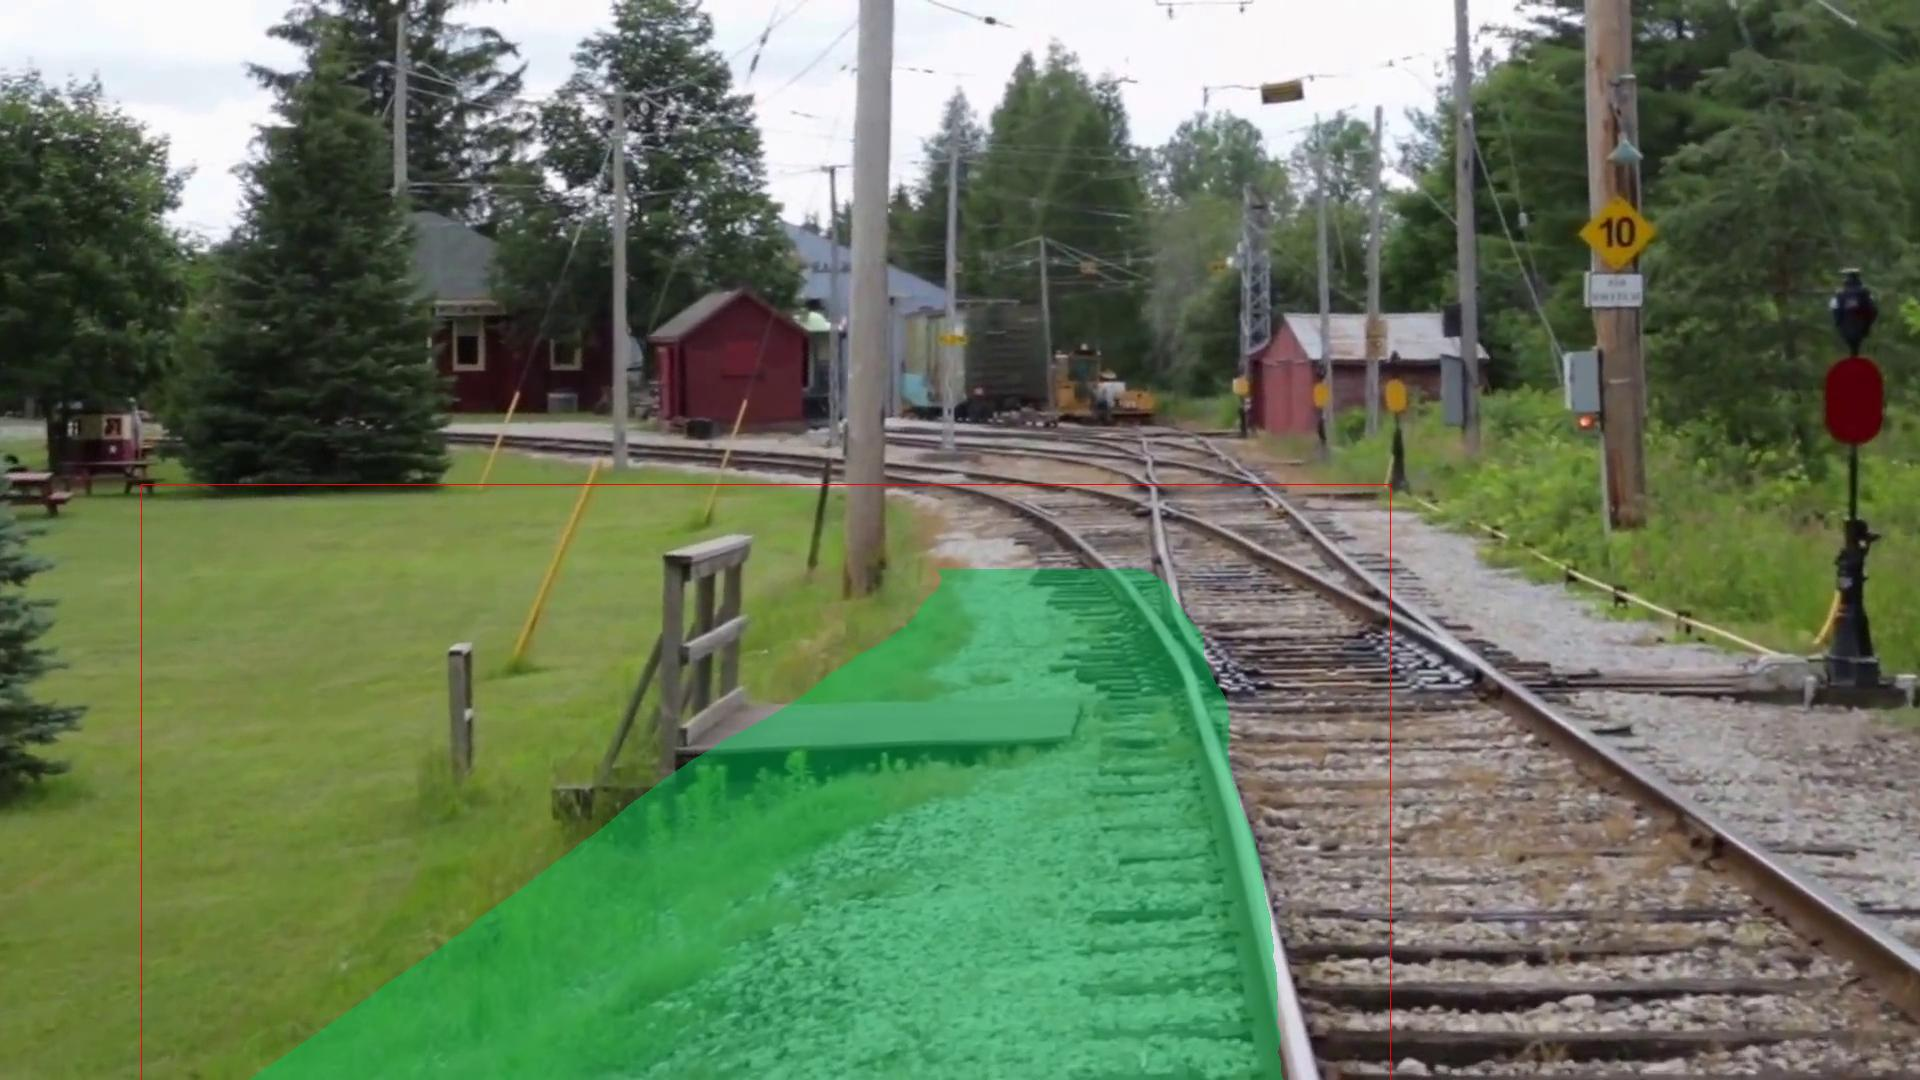
\includegraphics[width=\textwidth]{PICs/experiments/ComparisonBaselineToImproved/original2.jpg}
        \end{subfigure}
        \begin{subfigure}[b]{0.48\textwidth}
            \centering
            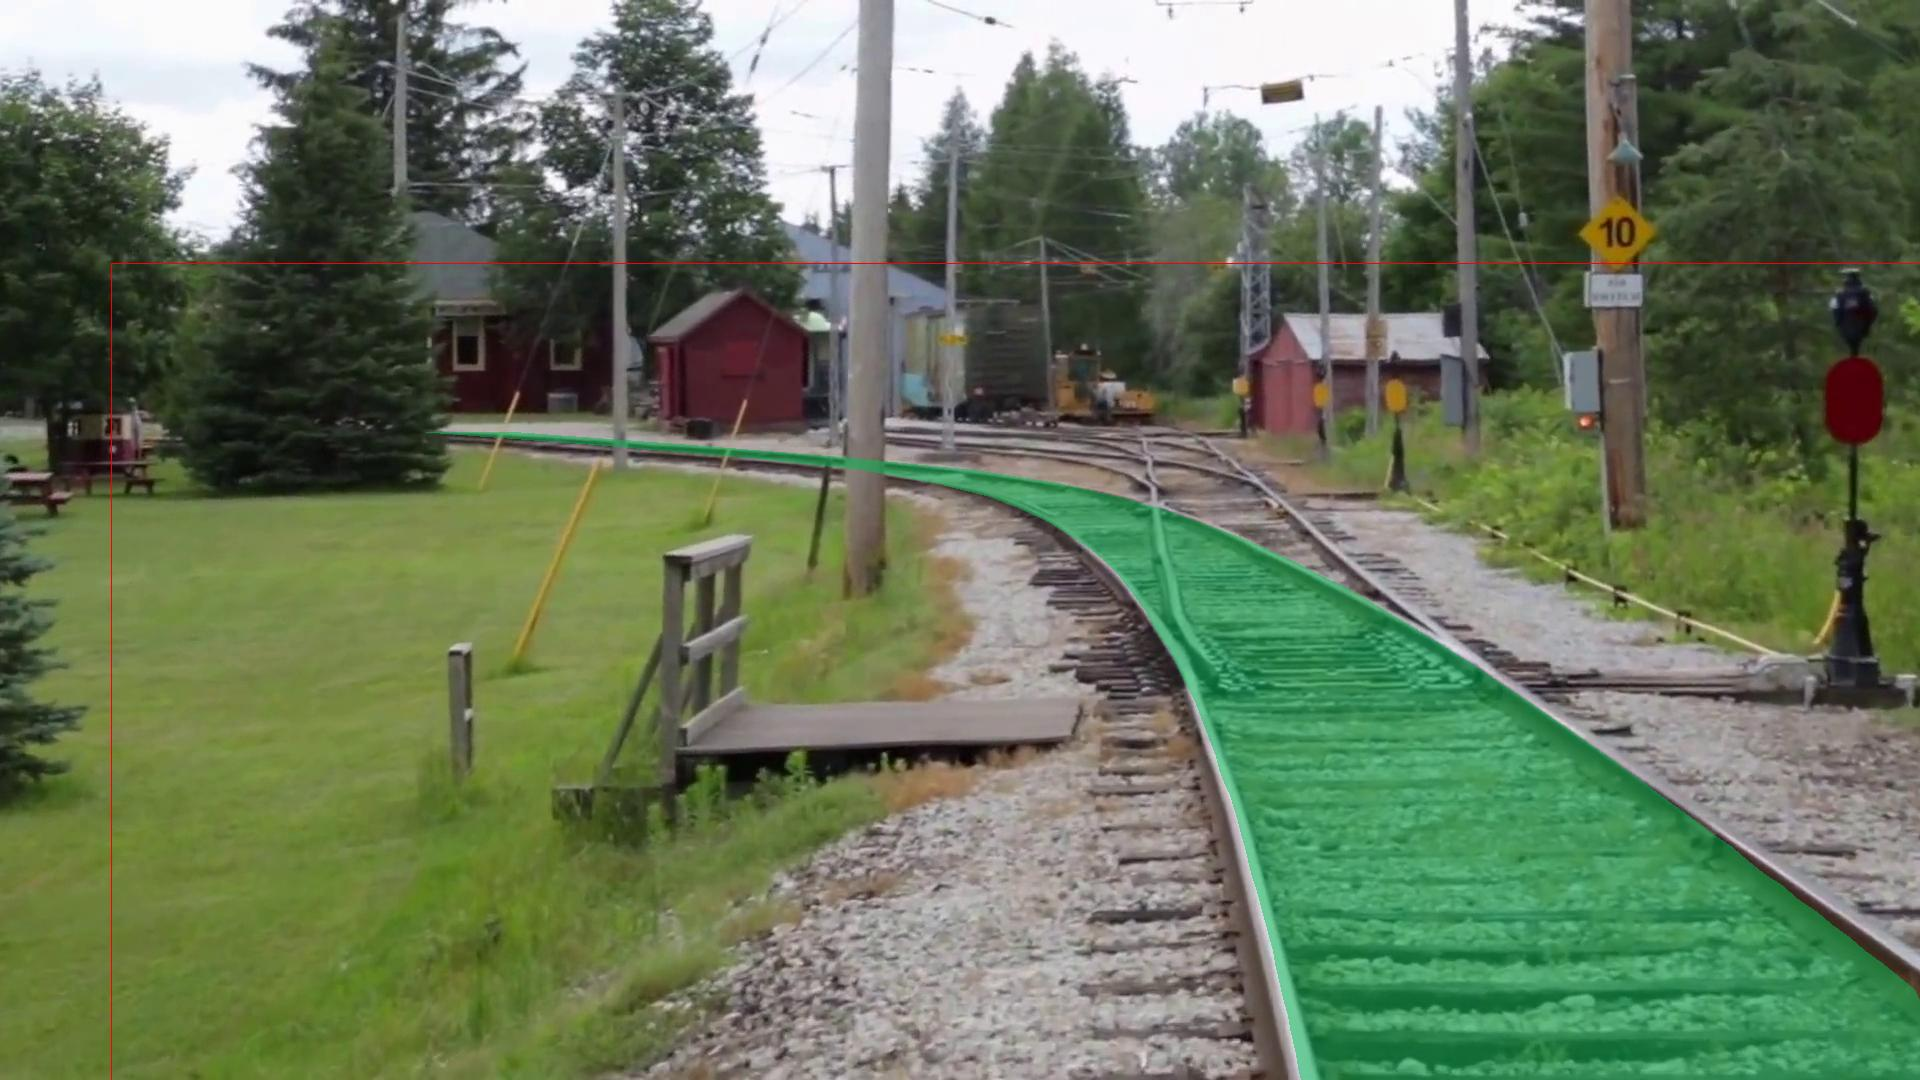
\includegraphics[width=\textwidth]{PICs/experiments/ComparisonBaselineToImproved/adapted2.jpg}
        \end{subfigure}
        
        \vspace{0.5cm} % Abstand zwischen den Zeilen
        
        \begin{subfigure}[b]{0.48\textwidth}
            \centering
            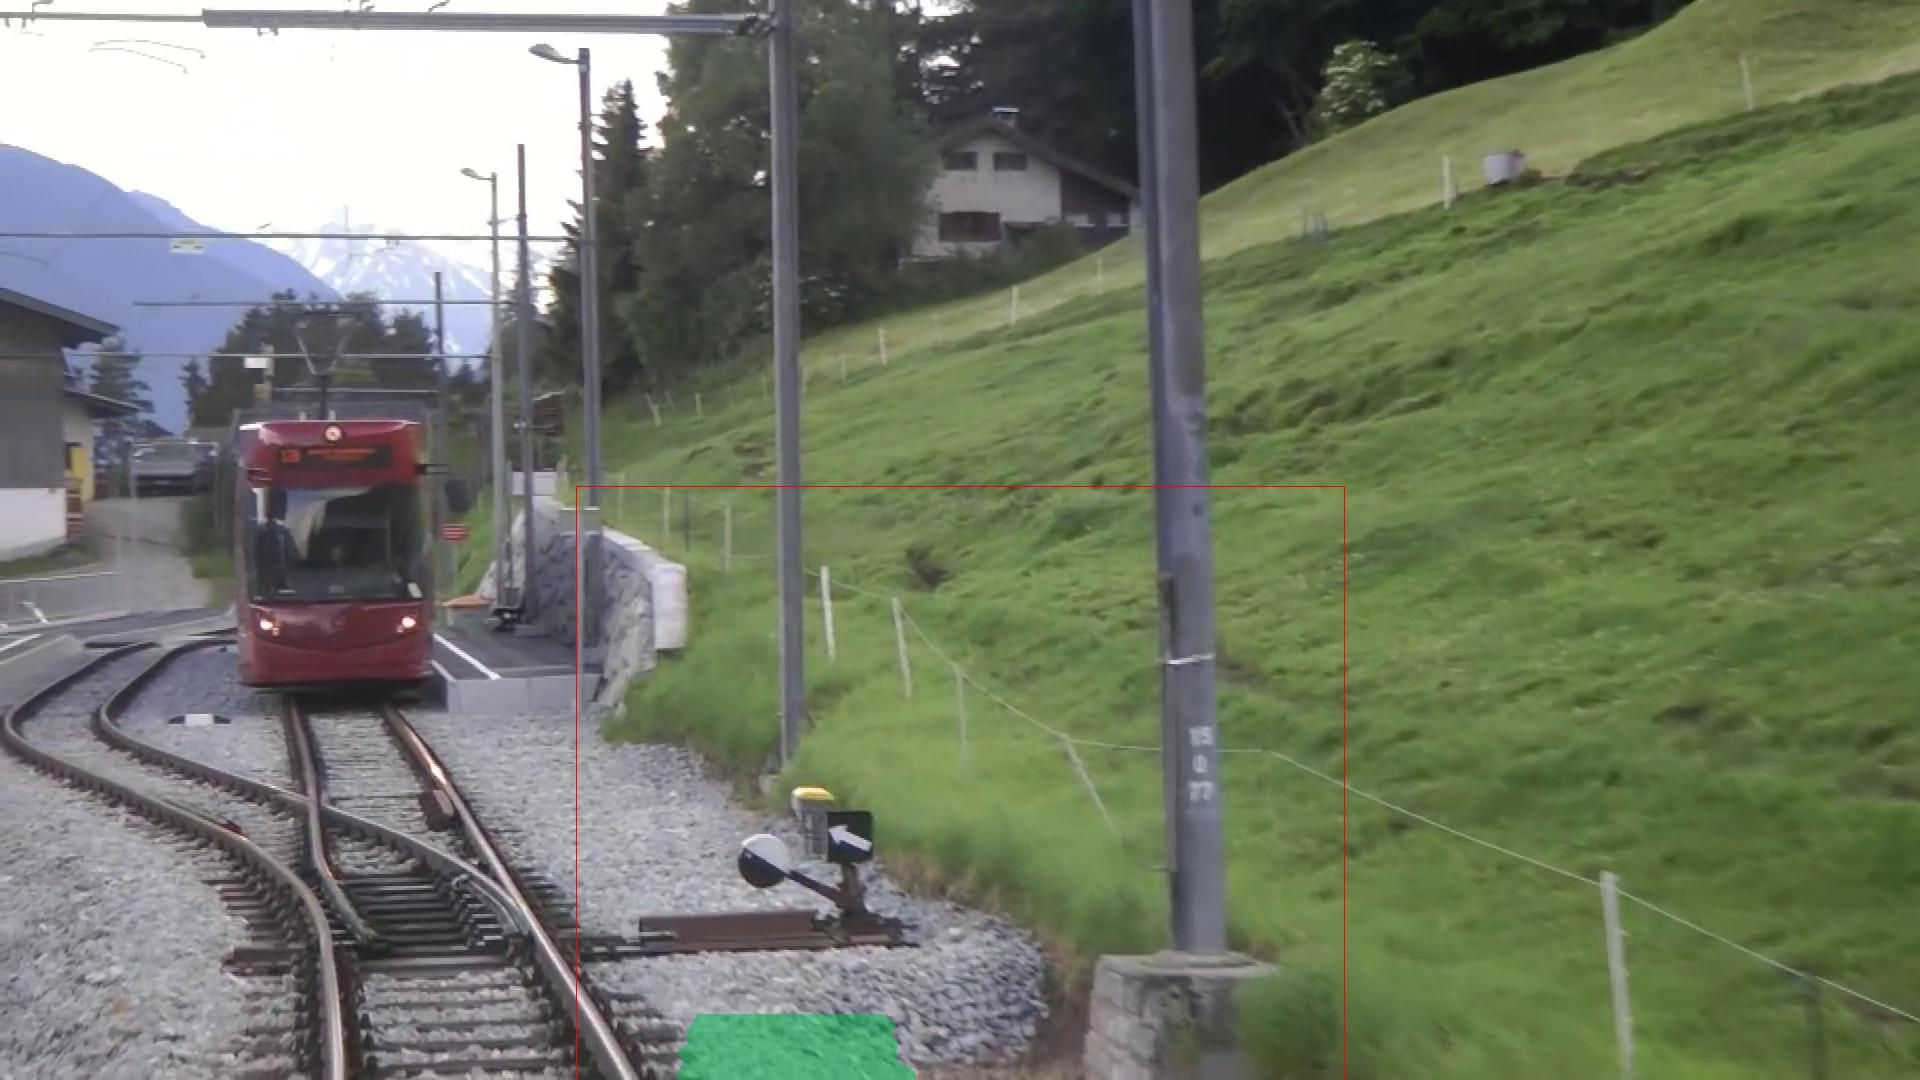
\includegraphics[width=\textwidth]{PICs/experiments/ComparisonBaselineToImproved/original1.jpg}
        \end{subfigure}
        \begin{subfigure}[b]{0.48\textwidth}
            \centering
            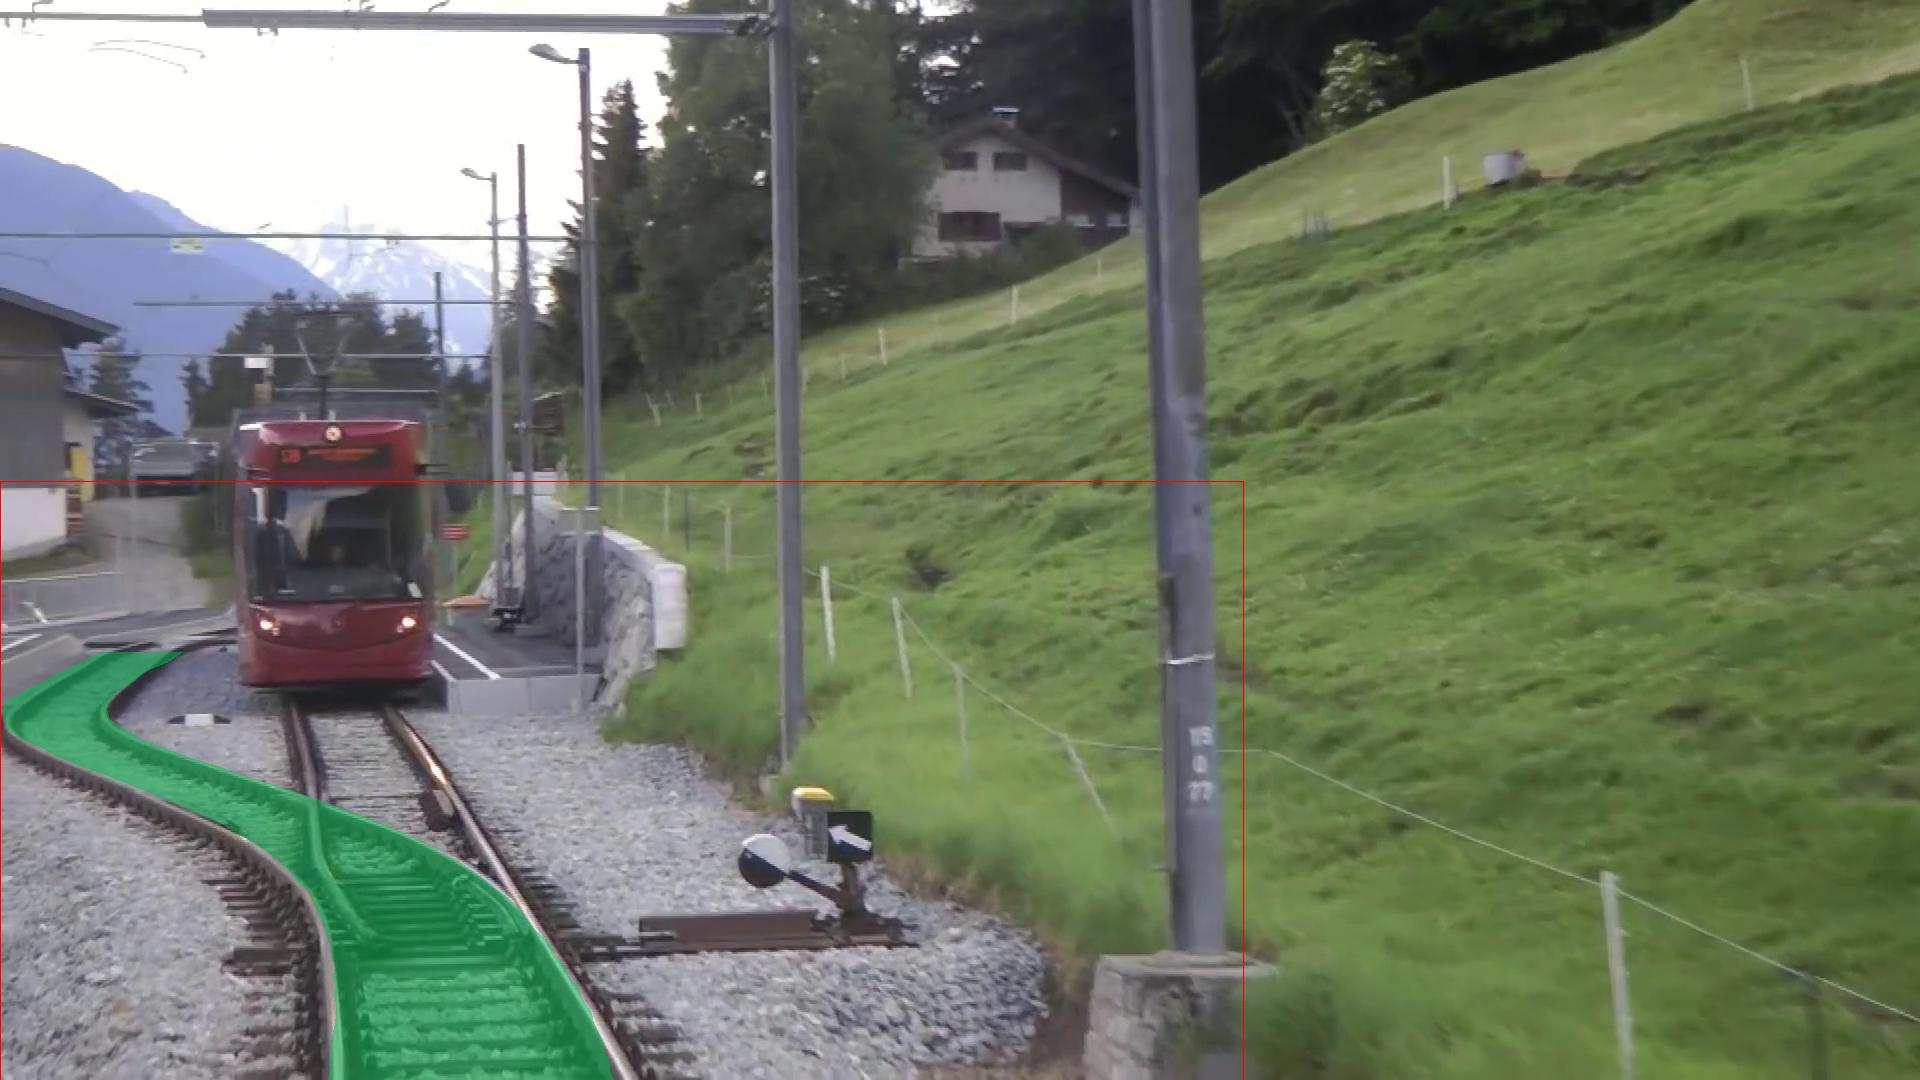
\includegraphics[width=\textwidth]{PICs/experiments/ComparisonBaselineToImproved/adapted1.jpg}
        \end{subfigure}
        
        \vspace{0.5cm} % Abstand zwischen den Zeilen
        
        \begin{subfigure}[b]{0.48\textwidth}
            \centering
            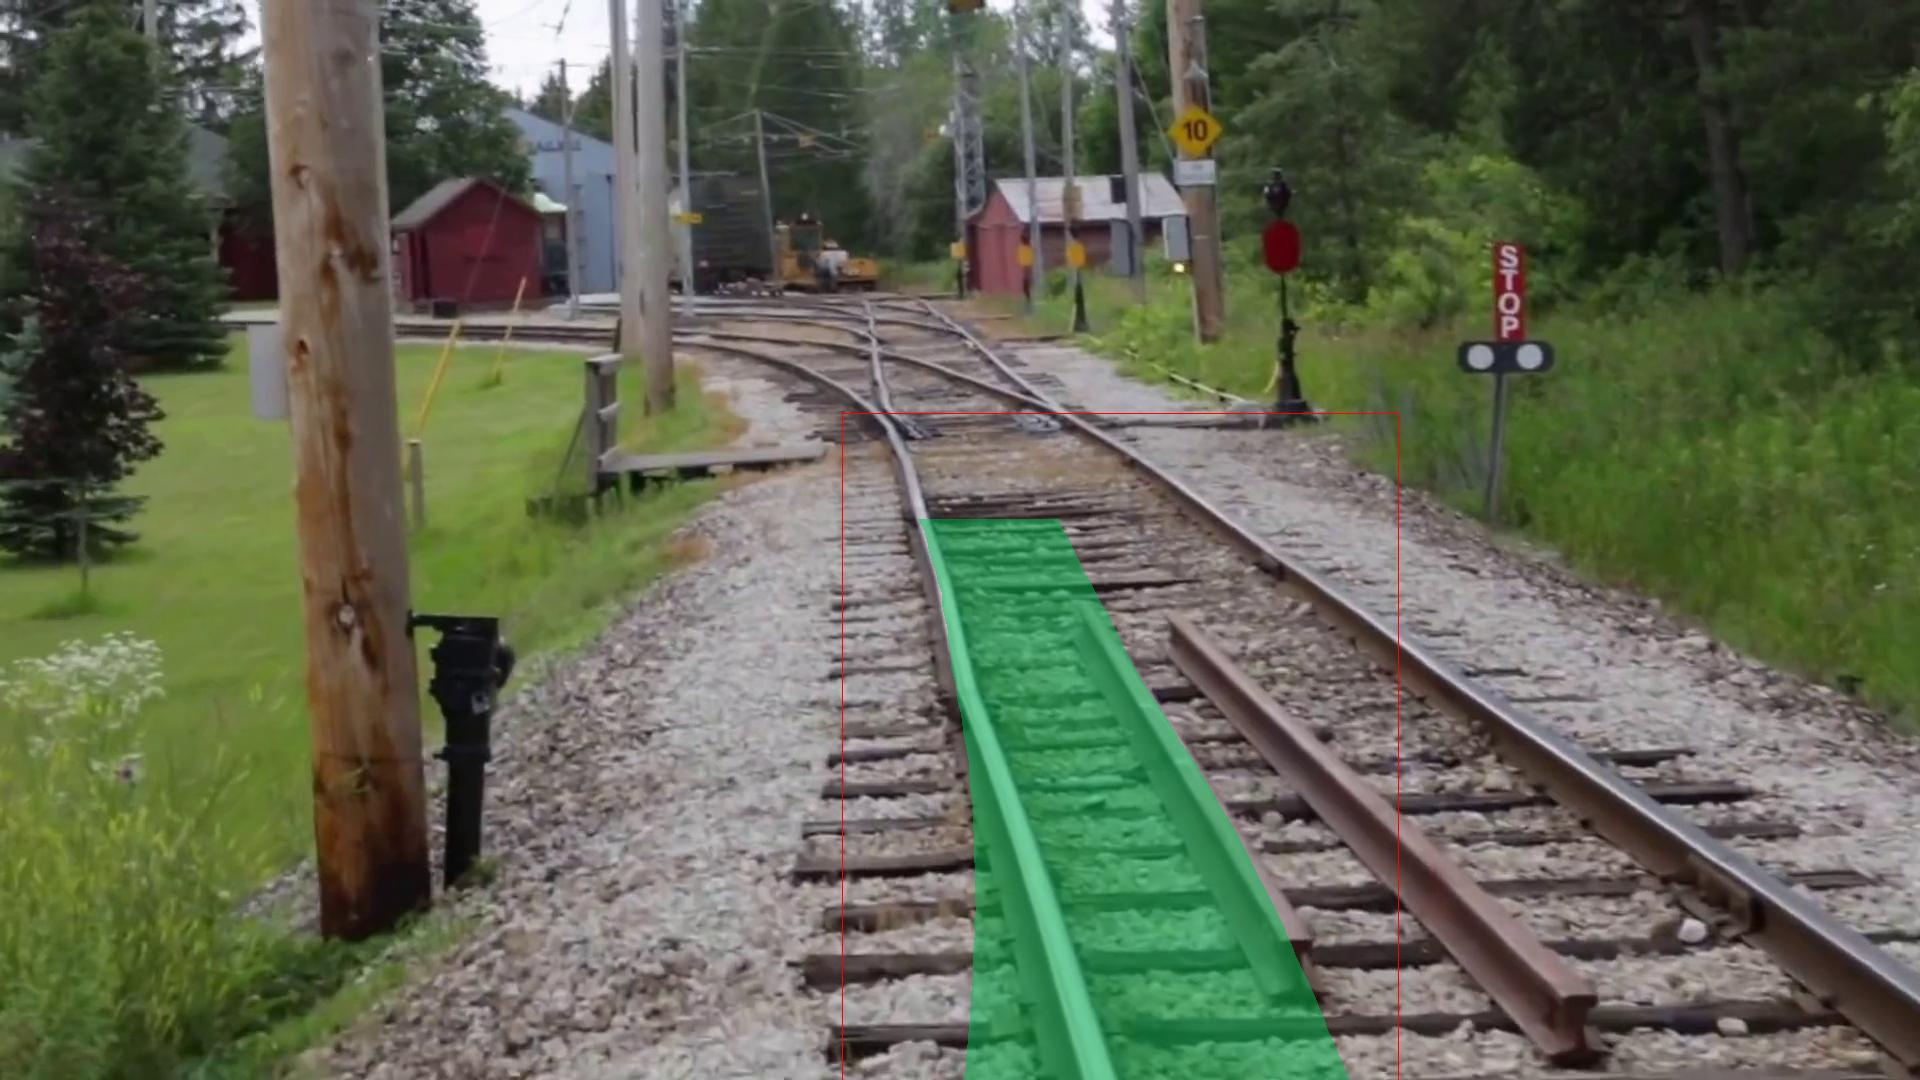
\includegraphics[width=\textwidth]{PICs/experiments/ComparisonBaselineToImproved/original3.jpg}
        \end{subfigure}
        \begin{subfigure}[b]{0.48\textwidth}
            \centering
            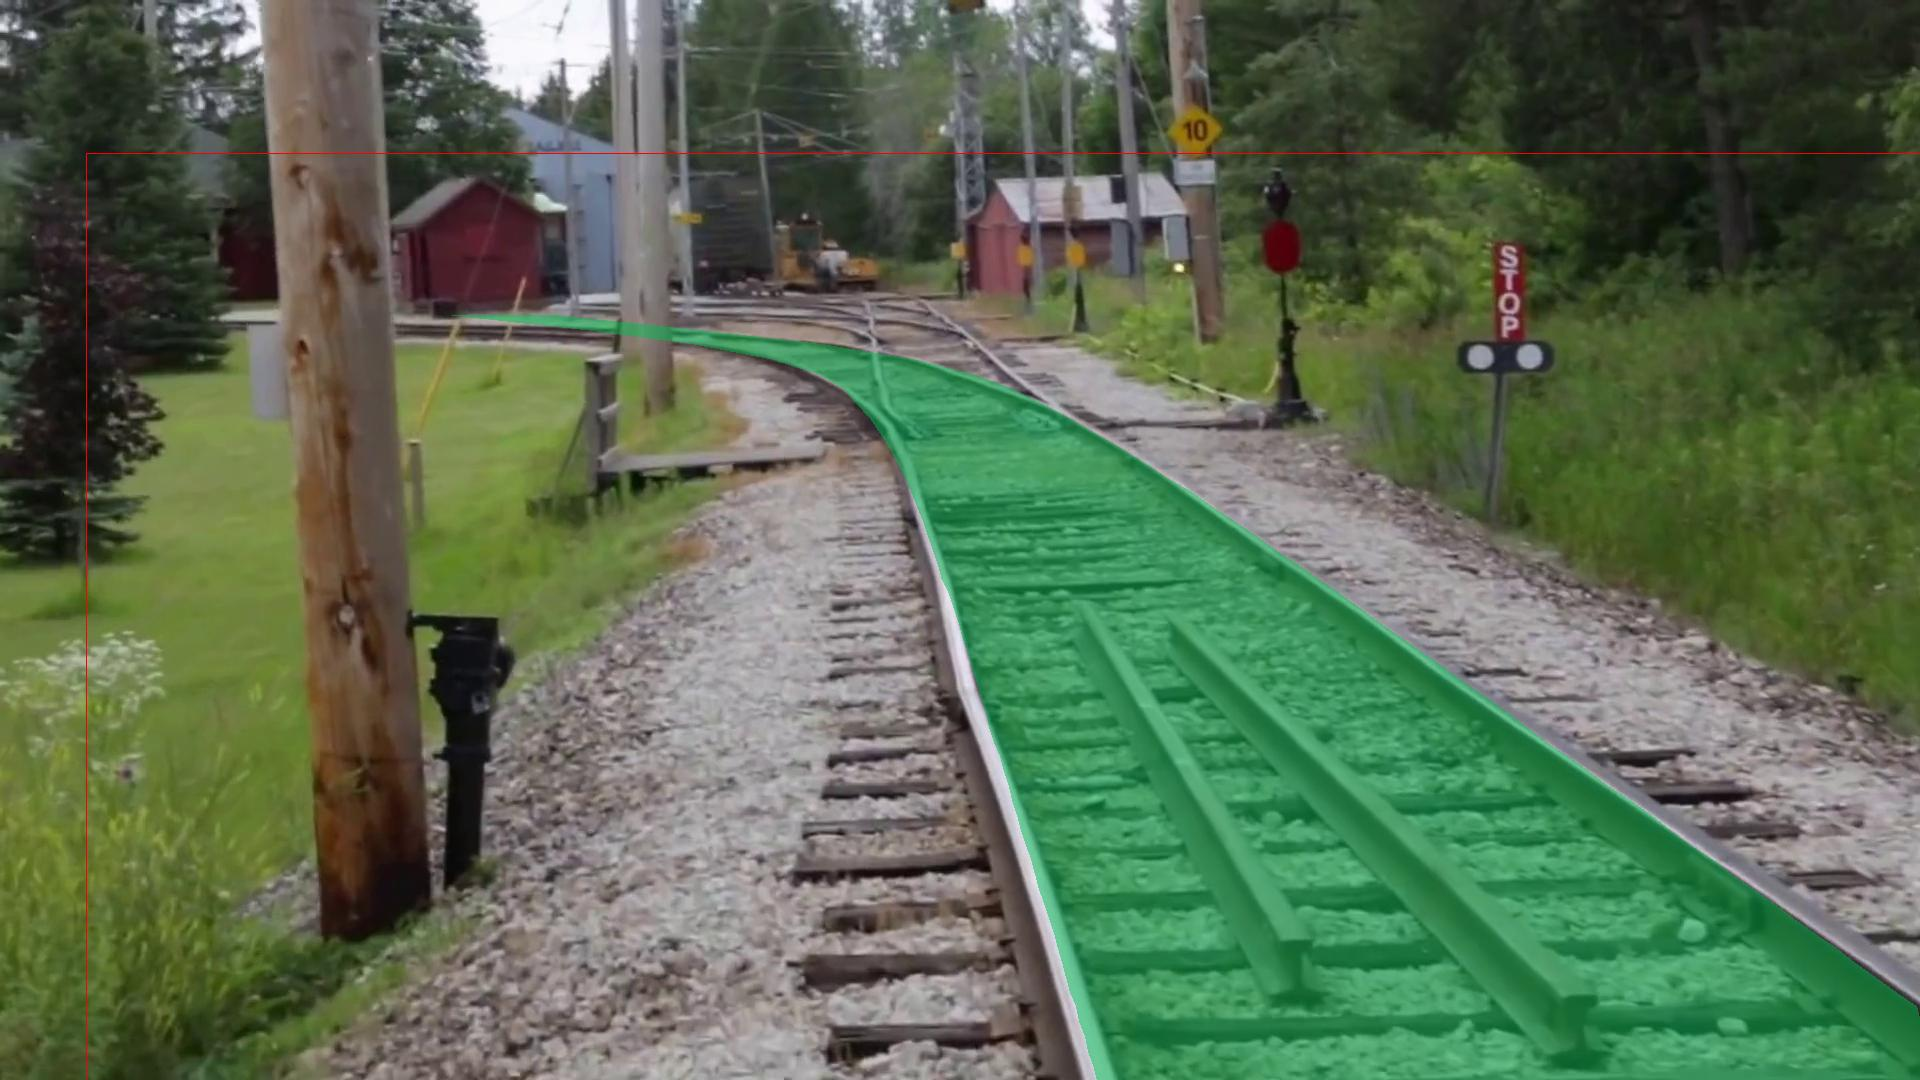
\includegraphics[width=\textwidth]{PICs/experiments/ComparisonBaselineToImproved/adapted3.jpg}
        \end{subfigure}
    \end{minipage}%
    \hfill
    \begin{minipage}{0.2\textwidth} % Rechte Seite für Text
        \centering
        \textbf{adapted TEP-Net}\\
        EfficientNet-B3
    \end{minipage}
    \caption{Comparison between the best version of TEP-Net \cite{tepNet2024} and the best version with all improvements of this work: best backbone, adaptive max pooling, trapeze head, and adapted autocrop mechanism.
    Images of complex scenes with difficult angles of perspective are intentionally chosen.}
    \label{fig:comparisonBaseline2Improved}
\end{figure}

\autoref{fig:comparisonBaseline2Improved} shows three examples of the switch evaluation dataset.
These predictions are obtained with the autocrop mechanism.
The crop coordinates are adjusted by predicting each image 50 times.
On the left, predictions are made with the best-performing model from \cite{tepNet2024} with the original auto cropping technique, and on the right, all introduced improvements are used.
That includes the adapted auto crop mechanism and best-performing model incorporating an EfficientNet-B3 backbone, the adaptive max pooling layer, and the trapeze head.

For this brief qualitative comparison, three images with intentionally complex scenes are chosen to view differences more clearly.
That includes rails captured from very unusual angles that do not start from the bottom center like most other images from the dataset.
In the image in the bottom row, additional rails lay in the track, introducing an extra challenge.

\autoref{fig:comparisonBaseline2Improved} visualizes that the original model \cite{tepNet2024} struggles to find the track.
The improved version finds the track and correctly predicts the switch in each image, demonstrating that all introduced adaptations increase the system's robustness and thus enhance safety in a practical application.


%%%%%%%%%%%%%%%%%%%%%%%%%% Temporal Models %%%%%%%%%%%%%%%%%%%%%%%%%%

\subsection{Sliding Window Approach}
blindtext

\subsection{Temporal Models}
blindtext

\begin{table}[H]
    \centering
    \resizebox{\textwidth}{!}{
    \begin{tabular}{lcccccc}
        \hline
        \rowcolor{white} \textbf{Model} & \textbf{Parameters} & \textbf{Flops} & \textbf{MACs} & \textbf{Latency TRT FP32 / FP16} & \textbf{IoU} & \textbf{Switch Eval} \\
        \hline
        \rowcolor[gray]{0.9} single-frame-based          & xyM & xyB & xyG & xy / xy ms & 0.xy & xy \% \\ 
        \hline
        \rowcolor{white}     CNN\_LSTM\_FC               & xyM & xyB & xyG & xy / xy ms & 0.xy & xy \% \\ 
        \rowcolor[gray]{0.9} CNN\_FC\_LSTM               & xyM & xyB & xyG & xy / xy ms & 0.xy & xy \% \\ 
        \rowcolor{white}     CNN\_LSTM\_V1               & xyM & xyB & xyG & xy / xy ms & 0.xy & xy \% \\ 
        \rowcolor[gray]{0.9} CNN\_LSTM\_V2               & xyM & xyB & xyG & xy / xy ms & 0.xy & xy \% \\ 
        \rowcolor{white}     CNN\_LSTM\_HEAD             & xyM & xyB & xyG & xy / xy ms & 0.xy & xy \% \\ 
        \rowcolor[gray]{0.9} CNN\_FC\_FCOUT\_V1          & xyM & xyB & xyG & xy / xy ms & 0.xy & xy \% \\ 
        \rowcolor{white}     CNN\_FC\_FCOUT\_V2          & xyM & xyB & xyG & xy / xy ms & 0.xy & xy \% \\ 
        \rowcolor[gray]{0.9} CNN\_FLAT\_FC               & xyM & xyB & xyG & xy / xy ms & 0.xy & xy \% \\ 
        \rowcolor{white}     CNN\_LSTM\_SKIP\_CAT        & xyM & xyB & xyG & xy / xy ms & 0.xy & xy \% \\ 
        \rowcolor[gray]{0.9} CNN\_LSTM\_SKIP\_MUL\_FRAME & xyM & xyB & xyG & xy / xy ms & 0.xy & xy \% \\ 
        \rowcolor{white}     CNN\_LSTM\_SKIP\_MUL\_TIME  & xyM & xyB & xyG & xy / xy ms & 0.xy & xy \% \\ 
        \hline
    \end{tabular}
    }
    \caption{Temporal Models Results}
    \label{tab:temporalModelsResults}
\end{table}
